% ============================================================
% IEEE Conference Paper: Groundwater ML Under Extreme Conditions
% AFML Research Project — Person 4 Contribution
% Compile: latexmk -pdf main.tex
%          or: pdflatex main && bibtex main && pdflatex main && pdflatex main
% ============================================================
\documentclass[conference]{IEEEtran}

\usepackage{cite}
\usepackage{amsmath,amssymb}
\usepackage{graphicx}
\usepackage{booktabs}
\usepackage{array}
\usepackage{url}
\usepackage{hyperref}
\usepackage{xspace}
\usepackage{multirow}
\usepackage{siunitx}

% Convenience macros
\newcommand{\RF}{Random Forest\xspace}
\newcommand{\MAE}{MAE\xspace}
\newcommand{\RMSE}{RMSE\xspace}

\graphicspath{{figures/}}

% ============================================================
\begin{document}

\title{Machine Learning Performance Degradation Under Extreme
       Hydroclimatic Conditions: Input Extrapolation and Predictive
       Relationship Instability in Groundwater Level Prediction}

% Authors: placeholder block — real names/affiliations not public
\author{%
  \IEEEauthorblockN{Author One}
  \IEEEauthorblockA{Department of Computer Science\\
    University (Placeholder)\\
    Email: author1@placeholder.edu}
  \and
  \IEEEauthorblockN{Author Two}
  \IEEEauthorblockA{Department of Computer Science\\
    University (Placeholder)\\
    Email: author2@placeholder.edu}
  \and
  \IEEEauthorblockN{Author Three}
  \IEEEauthorblockA{Department of Computer Science\\
    University (Placeholder)\\
    Email: author3@placeholder.edu}
  \and
  \IEEEauthorblockN{Author Four}
  \IEEEauthorblockA{Department of Computer Science\\
    University (Placeholder)\\
    Email: author4@placeholder.edu}
}

\maketitle

% ============================================================
\begin{abstract}
Groundwater is a critical freshwater resource for drinking water,
agriculture, and industrial use, yet machine learning (ML) models for
groundwater-level prediction routinely underperform during extreme
hydroclimatic conditions.
Two mechanisms can contribute to this failure: \emph{input extrapolation},
in which test observations fall outside the region of the input feature
space covered by training data, and \emph{predictive relationship
instability}, in which prediction errors increase even when inputs remain
within previously encountered ranges.
Prior evaluation practice rarely separates these two explanations.

This paper investigates both mechanisms using a Random Forest regressor
trained on 87{,}426 quarterly groundwater observations from Karnataka,
India (Central Ground Water Board, 1996--2017) and evaluated on 14{,}863
held-out observations (2018--2020).
Input novelty is quantified by mean distance to the five nearest training
neighbours in standardised seven-dimensional feature space.

The Random Forest reduces mean absolute error (MAE) by 23.5\% and root
mean squared error (RMSE) by 21.2\% relative to a persistence baseline.
Test observations in the extreme-novelty group (above the 99th-percentile
novelty threshold) have an MAE of 3.34\,m, compared to 1.82\,m for
familiar observations---an increase of 83.9\%.
Environmental feature-space novelty (rainfall, prior groundwater level,
and seasonal features) explains substantially more of the error increase
than geographic novelty alone.
A paired temporal analysis of 1{,}516 wells reveals an MAE increase from
1.71\,m in 2018 to 2.13\,m in 2020, with a bootstrap 95\,\% CI of
$[+0.298, +0.531]$\,m excluding zero.
A within-well matched-input comparison (2{,}077 pairs, 1{,}311 wells)
shows a 0.51\,m increase with CI $[+0.410, +0.605]$\,m, suggesting that
temporal deterioration cannot be explained entirely by shifts in input
distributions.
An independent evaluation by a third team member (12/12 data integrity
checks passing) confirms all primary metrics.
Planned reliability-aware modelling was not completed, representing a
documented gap.
The findings suggest that both input extrapolation and temporal predictive
instability deserve attention when deploying ML groundwater models in
regions subject to hydroclimatic variability.
\end{abstract}

\begin{IEEEkeywords}
groundwater level prediction, machine learning, Random Forest, input
extrapolation, predictive relationship instability, distribution shift,
concept drift, hydroclimatic extremes, novelty detection, robustness
evaluation
\end{IEEEkeywords}

% ============================================================
\section{Introduction}
\label{sec:intro}

Groundwater constitutes a large fraction of global accessible freshwater
and underpins food security, rural drinking water supply, and industrial
processes in many developing regions \cite{famiglietti2014groundwater}.
In India, groundwater accounts for a substantial portion of irrigation
withdrawals, and declining aquifer levels in several states have been
linked to both over-extraction and reduced recharge under changing
precipitation regimes \cite{rodell2009satellite}.

Machine learning methods have attracted sustained interest as a
complement or alternative to physics-based groundwater models.
Random Forests and gradient boosted trees are frequently reported to
achieve lower prediction errors than conventional regression on
groundwater-level data \cite{rajaee2019review, wunsch2021groundwater}.
However, standard evaluation practice focuses on overall held-out metrics
and rarely examines model behaviour during the specific conditions---high
rainfall, drought, rapid recharge events---that are most relevant for
water management decisions.

Two distinct mechanisms can cause an ML model to perform poorly under
extreme conditions.
First, test observations may contain combinations of input features that
are poorly supported by the training distribution, forcing the model to
extrapolate beyond the region in which it was fitted \cite{quionero2009dataset}.
Second, the learned predictive relationship between inputs and outputs may
itself change over time due to concept drift---shifts in the conditional
distribution $P(y \mid \mathbf{x})$ not captured by changes in
$P(\mathbf{x})$ alone \cite{gama2014survey}.
Separating these two explanations is both scientifically important and
practically relevant: input extrapolation suggests the need for more
representative training data or explicit out-of-distribution detection,
while predictive relationship instability points toward retraining
schedules, ensemble diversity, or uncertainty-aware modelling.

This paper addresses the central research question: \emph{when groundwater
ML models fail under extreme hydroclimatic conditions, to what extent can
the degradation be associated with unfamiliar inputs versus instability in
predictive performance under otherwise familiar inputs?}

The main contributions of this work are:
\begin{enumerate}
  \item A nearest-neighbour novelty framework applied to a large
        groundwater dataset to quantify input extrapolation and its
        association with prediction errors.
  \item A decomposition of novelty by feature type (geographic,
        environmental, and combined), showing that environmental novelty
        drives the error increase while geographic distance does not.
  \item Paired temporal and matched-input analyses establishing that
        prediction errors increased between 2018 and 2020 in a manner
        that is not fully explained by input distribution changes.
  \item A temporal residual regression demonstrating that the
        relationship between model errors and input features changes
        across years.
  \item A controlled training-removal experiment probing the causal
        link between rare training observations and model support for
        unfamiliar test inputs.
  \item An independent, third-party evaluation confirming all primary
        metrics with 12/12 data integrity checks passing.
  \item Transparent documentation of a planned reliability-aware
        modelling component that was not completed.
\end{enumerate}

% ============================================================
\section{Related Work}
\label{sec:related}

\subsection{Machine Learning for Groundwater Prediction}

Data-driven methods for groundwater level (GWL) prediction have been
reviewed comprehensively by Rajaee et al.~\cite{rajaee2019review}, who
document that artificial neural networks and ensemble methods frequently
outperform autoregressive statistical models on regional datasets.
Wunsch et al.~\cite{wunsch2021groundwater} demonstrate that long
short-term memory (LSTM) networks can capture temporal dependencies in
GWL time series across diverse hydrogeological settings.
Sahoo et al.~\cite{sahoo2017machine} compare several ML methods
including Random Forest, support vector regression, and multilayer
perceptron on shallow aquifer data, finding that Random Forest provides
competitive accuracy with lower sensitivity to hyperparameter choice.
Breiman's original Random Forest formulation \cite{breiman2001random}
remains the foundation for the ensemble approach used here, and
scikit-learn~\cite{pedregosa2011scikit} provides the implementation.

\subsection{Hydroclimatic Extremes and Groundwater}

Rodell et al.~\cite{rodell2009satellite} use GRACE satellite observations
to show declining groundwater storage in northern India linked to
monsoon variability and over-extraction.
Extreme precipitation can cause rapid recharge that overwhelms model
predictions trained on moderate conditions \cite{wunsch2021groundwater}.
The mismatch between training distributions and extreme-event conditions
has been identified as a key limitation of static ML models in
hydrology \cite{rajaee2019review}.

\subsection{Distribution Shift and Input Extrapolation}

The general framework for covariate shift and dataset shift is set out in
Quionero-Candela et al.~\cite{quionero2009dataset}.
Under covariate shift, the marginal distribution of inputs $P(\mathbf{x})$
differs between training and test, while the conditional $P(y|\mathbf{x})$
remains stable.
Techniques for detecting and correcting for covariate shift in supervised
learning include importance weighting, kernel mean matching, and
nearest-neighbour distance measures~\cite{quionero2009dataset}.
The novelty measure used in the present work---mean distance to the $k$
nearest training neighbours in standardised feature space---is a
simple, model-agnostic proxy for the degree of input extrapolation.

\subsection{Concept Drift and Predictive Relationship Instability}

Gama et al.~\cite{gama2014survey} provide a comprehensive survey of
concept drift detection and adaptation methods, distinguishing sudden,
gradual, recurring, and incremental drift.
In the groundwater context, slow changes in aquifer behaviour, land use,
and measurement practice could contribute to gradual drift that is not
captured by seasonal and rainfall features alone.
The temporal residual regression approach used in Section~\ref{sec:method}
draws on the fixed-effects panel regression framework, treating well
identity as a grouping variable to separate within-well temporal change
from between-well heterogeneity.

\subsection{Reliability-Aware ML and Prediction Intervals}

Conformal prediction provides distribution-free coverage guarantees for
prediction intervals under exchangeability
conditions \cite{vovk2005algorithmic}.
Interval-based evaluation complements point-error metrics by quantifying
predictive uncertainty, which is particularly important when models are
used for risk-sensitive water-management decisions.
The planned reliability-aware component of this study aimed to construct
and evaluate prediction intervals; as documented in
Section~\ref{sec:method}, the corresponding result files were not
produced.

\subsection{Robustness Evaluation}

Standard held-out evaluation may understate performance degradation on
rare or extreme observations if those observations are a small fraction
of the test set.
Grouped evaluation, within-unit comparisons, and bootstrap confidence
intervals provide more targeted assessments of robustness \cite{efron1993bootstrap}.
Bootstrap resampling at the well (cluster) level, as used here, accounts
for within-well correlation in time-series groundwater data.

% ============================================================
\section{Dataset and Study Design}
\label{sec:data}

\subsection{Data Source}

The primary dataset is derived from Central Ground Water Board (CGWB)
quarterly groundwater observation records for Karnataka, India.
The raw processed dataset (\texttt{groundwater\_rainfall\_features\_qc.csv})
contains 104{,}781 observations across 30 columns, covering station
identifiers, geographical coordinates, GWL measurements, observation
dates, 30-day and 90-day accumulated rainfall, and quality-control flags.

\subsection{Target Variable and Feature Construction}

The prediction target is \emph{Groundwater Level Quarterly Manual
(meter)}, measured as depth below ground surface.
Seven input features are used for modelling (Table~\ref{tab:features}).

\begin{table}[htbp]
\centering
\caption{Input Features Used in the Random Forest Model}
\label{tab:features}
\begin{tabular}{@{}ll@{}}
\toprule
\textbf{Feature} & \textbf{Description} \\
\midrule
Latitude & Station geographical latitude \\
Longitude & Station geographical longitude \\
\texttt{rainfall\_30d\_mm} & 30-day accumulated rainfall (mm) \\
\texttt{rainfall\_90d\_mm} & 90-day accumulated rainfall (mm) \\
\texttt{previous\_gwl} & Previous GWL observation, same well \\
\texttt{month\_sin} & Sine encoding of observation month \\
\texttt{month\_cos} & Cosine encoding of observation month \\
\bottomrule
\end{tabular}
\end{table}

A unique well identifier is constructed from station name, latitude, and
longitude.
Observations are sorted chronologically within each well, and
\texttt{previous\_gwl} is the immediately preceding GWL observation for
the same well.
The month is encoded using sine and cosine projections to represent
its cyclical nature.
Rows without a valid previous observation are excluded, yielding
102{,}289 usable rows.

\subsection{Train/Test Split}

A chronological split is applied at 2018-01-01:

\begin{itemize}
  \item \textbf{Training:} 87{,}426 observations (1996-05-15 to 2017-11-05)
  \item \textbf{Testing:} 14{,}863 observations (2018-01-05 to 2020-11-30)
\end{itemize}

The test set is strictly held out for evaluation.
No model parameters, novelty thresholds, or preprocessing transformations
are fitted using test data.

\subsection{Data Quality}

A data quality audit (Table~\ref{tab:data_quality}) identified 746 rows
with missing rainfall values (0.712\,\%), 57 observations with negative
GWL (0.054\,\%), and 256 observations with GWL above 50\,m (0.244\,\%).
Eight training observations have suspicious 30-day rainfall flags and 16
have suspicious 90-day rainfall flags; none of these flags occur in the
test period.
The sensitivity analysis in Section~\ref{sec:results} confirms that
excluding flagged training rows produces a negligible change in test
metrics ($\Delta$MAE $<$ 0.001\,m).

\begin{table}[htbp]
\centering
\caption{Data Quality Summary (104,781 total observations)}
\label{tab:data_quality}
\begin{tabular}{@{}lrr@{}}
\toprule
\textbf{Check} & \textbf{Count} & \textbf{Percentage} \\
\midrule
Missing target values & 0 & 0.000\,\% \\
Missing rainfall (30d or 90d) & 746 & 0.712\,\% \\
Duplicate well--date keys & 0 & 0.000\,\% \\
Negative GWL values & 57 & 0.054\,\% \\
GWL above 50\,m & 256 & 0.244\,\% \\
Suspicious rainfall 30d & 8 & 0.008\,\% \\
Suspicious rainfall 90d & 16 & 0.015\,\% \\
\bottomrule
\end{tabular}
\end{table}

% ============================================================
\section{Methodology}
\label{sec:method}

\subsection{Baseline Groundwater Prediction Models}

Two models are evaluated as baselines.

\textbf{Persistence baseline:} Predicts the next GWL measurement as equal
to the previous measurement for the same well.
This is a natural lower bound for a model using \texttt{previous\_gwl}
as a feature.

\textbf{Random Forest Regressor:} Configured with
$n\_\text{estimators} = 300$,
$\text{min\_samples\_leaf} = 3$,
$\text{random\_state} = 42$, and
$n\_\text{jobs} = -1$.
Scikit-learn 1.9.1 is used \cite{pedregosa2011scikit}.
The \texttt{StandardScaler} fitted on the training set is applied before
computing novelty scores (see below) but the Random Forest itself
operates on unscaled features.

\subsection{Input Extrapolation Analysis}

\textbf{Novelty score.}
For each test observation $\mathbf{x}_{\text{test}}$, its novelty score
is defined as the mean Euclidean distance to its five nearest neighbours
in the training set, computed in the standardised seven-feature space.
The \texttt{StandardScaler} is fitted on training data only.

\textbf{Novelty groups.}
The 95th and 99th percentiles of the novelty scores of training
observations (computed on training data) define three groups:
\begin{enumerate}
  \item \textit{Familiar:} novelty score $\leq 0.350078$ (95th percentile).
  \item \textit{Poorly represented:} $0.350078 <$ score $\leq 0.554389$ (99th percentile).
  \item \textit{Extreme novelty:} score $> 0.554389$.
\end{enumerate}

\textbf{Confidence intervals.}
Well-level cluster bootstrap resampling (2{,}000 repetitions, seed 42) is
used to estimate 95\,\% CIs for group MAE differences \cite{efron1993bootstrap}.
All observations from a sampled well are retained together, preserving
within-well correlation.

\textbf{Novelty type comparison.}
Three novelty definitions are compared: geographic (latitude, longitude),
environmental (rainfall, previous GWL, seasonal features), and combined
(all seven features).
Quartile groups are used rather than percentile thresholds to ensure equal
cell counts.

\textbf{Rainfall-only novelty.}
A separate analysis uses only \texttt{rainfall\_30d\_mm} and
\texttt{rainfall\_90d\_mm} to quantify novelty, testing whether the
full-feature error increase can be attributed to rainfall inputs alone.

\subsection{Predictive Relationship Instability}

\textbf{Conditional residual analysis.}
Random Forest residuals are computed for each test observation and
examined within bins of individual input features (30-day rainfall,
90-day rainfall, previous GWL) separately for 2018, 2019, and 2020.
This provides a qualitative view of how the error profile changes across
years within individual input ranges.

\textbf{Paired temporal comparison.}
For each well with observations in both 2018 and 2020, per-well MAE is
computed for each year.
The signed difference (2020 minus 2018) is bootstrapped at the well level
(2{,}000 repetitions) to estimate a 95\,\% CI for the mean temporal change.
1{,}516 wells qualify.

\textbf{Within-well matched-input comparison.}
Within each well, observations from 2018 and 2020 are matched one-to-one
by minimising distance across five input features
(\texttt{rainfall\_30d\_mm}, \texttt{rainfall\_90d\_mm},
\texttt{previous\_gwl}, \texttt{month\_sin}, \texttt{month\_cos}).
Only pairs within a maximum distance are retained, yielding 2{,}077 pairs
across 1{,}311 wells.
The error increase within matched pairs is bootstrapped at the well level.

\textbf{Temporal residual regression.}
Well fixed effects are absorbed by within-well demeaning.
Three OLS models are fitted on the demeaned residuals of the 12{,}142
observations belonging to wells represented in all three test years
(1{,}479 wells):
\begin{enumerate}
  \item Inputs only.
  \item Inputs $+$ year indicators.
  \item Inputs $+$ year indicators $+$ year $\times$ feature interactions.
\end{enumerate}
The improvement in $R^{2}$ from model (1) to model (3) measures the
additional explanatory power of year-dependent input--residual
relationships.

\textbf{Controlled training-removal experiment.}
Three Random Forest models are trained:
(A) on the full training set,
(B) with the top 1\,\% most locally novel training observations removed
(\emph{extreme-removed}), and
(C) with the same number of non-extreme training observations removed,
matched by year (\emph{matched-control}).
Test predictions from all three models are compared by test-novelty group
using well-level cluster bootstrap CIs (5{,}000 repetitions).

\subsection{Reliability-Aware Modelling (Person 2 — Absent)}
\label{sec:method:p2}

The planned reliability-aware modelling component was assigned to
Person 2 and aimed to produce prediction intervals, conformal coverage
evaluation, and interval width analysis under familiar and unfamiliar
conditions.
The corresponding result files---\texttt{reliability\_metrics.csv},
\texttt{reliability\_predictions.csv},
\texttt{reliability\_by\_condition.csv}, and
\texttt{reliability\_sensitivity.csv}---are absent from the repository.
No Person 2 results are available and none are presented in this paper.
This represents a documented gap in the study: prediction interval
calibration and conformal coverage cannot be evaluated.

\subsection{Independent Robustness Evaluation (Person 3)}
\label{sec:method:p3}

An independent evaluation was conducted to verify the primary results and
probe potential methodological issues.
The evaluation covered:
\begin{enumerate}
  \item \textbf{Data integrity:} 12 checks for duplicate well--date pairs,
        training-test overlap, missing predictions, and metric agreement.
        All 12 checks pass.
  \item \textbf{Grouped evaluation:} Familiar vs.\ unfamiliar conditions
        using training-derived rainfall bounds (5th--95th and 1st--99th
        percentiles of training rainfall).
  \item \textbf{Same-well paired analysis:} 386 wells with observations
        in both high-rainfall and normal conditions; per-well MAE
        differences bootstrapped (2{,}000 reps, well-level cluster).
  \item \textbf{Bootstrap CI verification:} Key CIs independently
        re-implemented with different seeds; agreement within 0.005\,m.
  \item \textbf{Rainfall QC sensitivity:} Evaluation-filter and retrain
        experiments for suspicious rainfall observations.
  \item \textbf{Date-column audit:} Two scripts (\texttt{full\_support\_analysis.py},
        \texttt{paired\_gwl\_support.py}) were found to use a different
        date column (\texttt{Data Acquisition Time}) and corrected to
        \texttt{observation\_date}, updating affected results.
  \item \textbf{Between-well confound diagnosis:} The apparently lower MAE
        of high-rainfall observations in unpaired comparisons is explained
        by systematic differences between wells that experience
        high-rainfall events and those that do not.
\end{enumerate}
Six comparison figures were generated and are included in this paper.

% ============================================================
\section{Experimental Results}
\label{sec:results}

\subsection{Baseline Performance}

Table~\ref{tab:baseline} reports overall test-set performance.
The Random Forest achieves MAE = 1.990\,m and RMSE = 3.498\,m with
$R^{2} = 0.769$, reducing MAE by 23.5\,\% and RMSE by 21.2\,\% relative
to the persistence baseline.
Figure~\ref{fig:baseline} shows a side-by-side comparison of prediction
errors.
Person 3's independent recalculation (Table~\ref{tab:p3metrics}) confirms
these values to machine precision.

\begin{table}[htbp]
\centering
\caption{Baseline Model Performance on the Test Set (n = 14,863)}
\label{tab:baseline}
\begin{tabular}{@{}lrrr@{}}
\toprule
\textbf{Model} & \textbf{MAE (m)} & \textbf{RMSE (m)} & \textbf{R\textsuperscript{2}} \\
\midrule
Persistence baseline & 2.6013 & 4.4389 & 0.6280 \\
Random Forest        & 1.9901 & 3.4977 & 0.7690 \\
\bottomrule
\end{tabular}
\end{table}

\begin{table}[htbp]
\centering
\caption{Person 3 Independent Verification Metrics (12/12 Data Checks PASS)}
\label{tab:p3metrics}
\begin{tabular}{@{}lrrr@{}}
\toprule
\textbf{Model} & \textbf{MAE (m)} & \textbf{RMSE (m)} & \textbf{R\textsuperscript{2}} \\
\midrule
Persistence baseline & 2.6013 & 4.4389 & 0.6280 \\
Random Forest        & 1.9901 & 3.4977 & 0.7690 \\
\bottomrule
\end{tabular}
\end{table}

\begin{figure}[htbp]
  \centering
  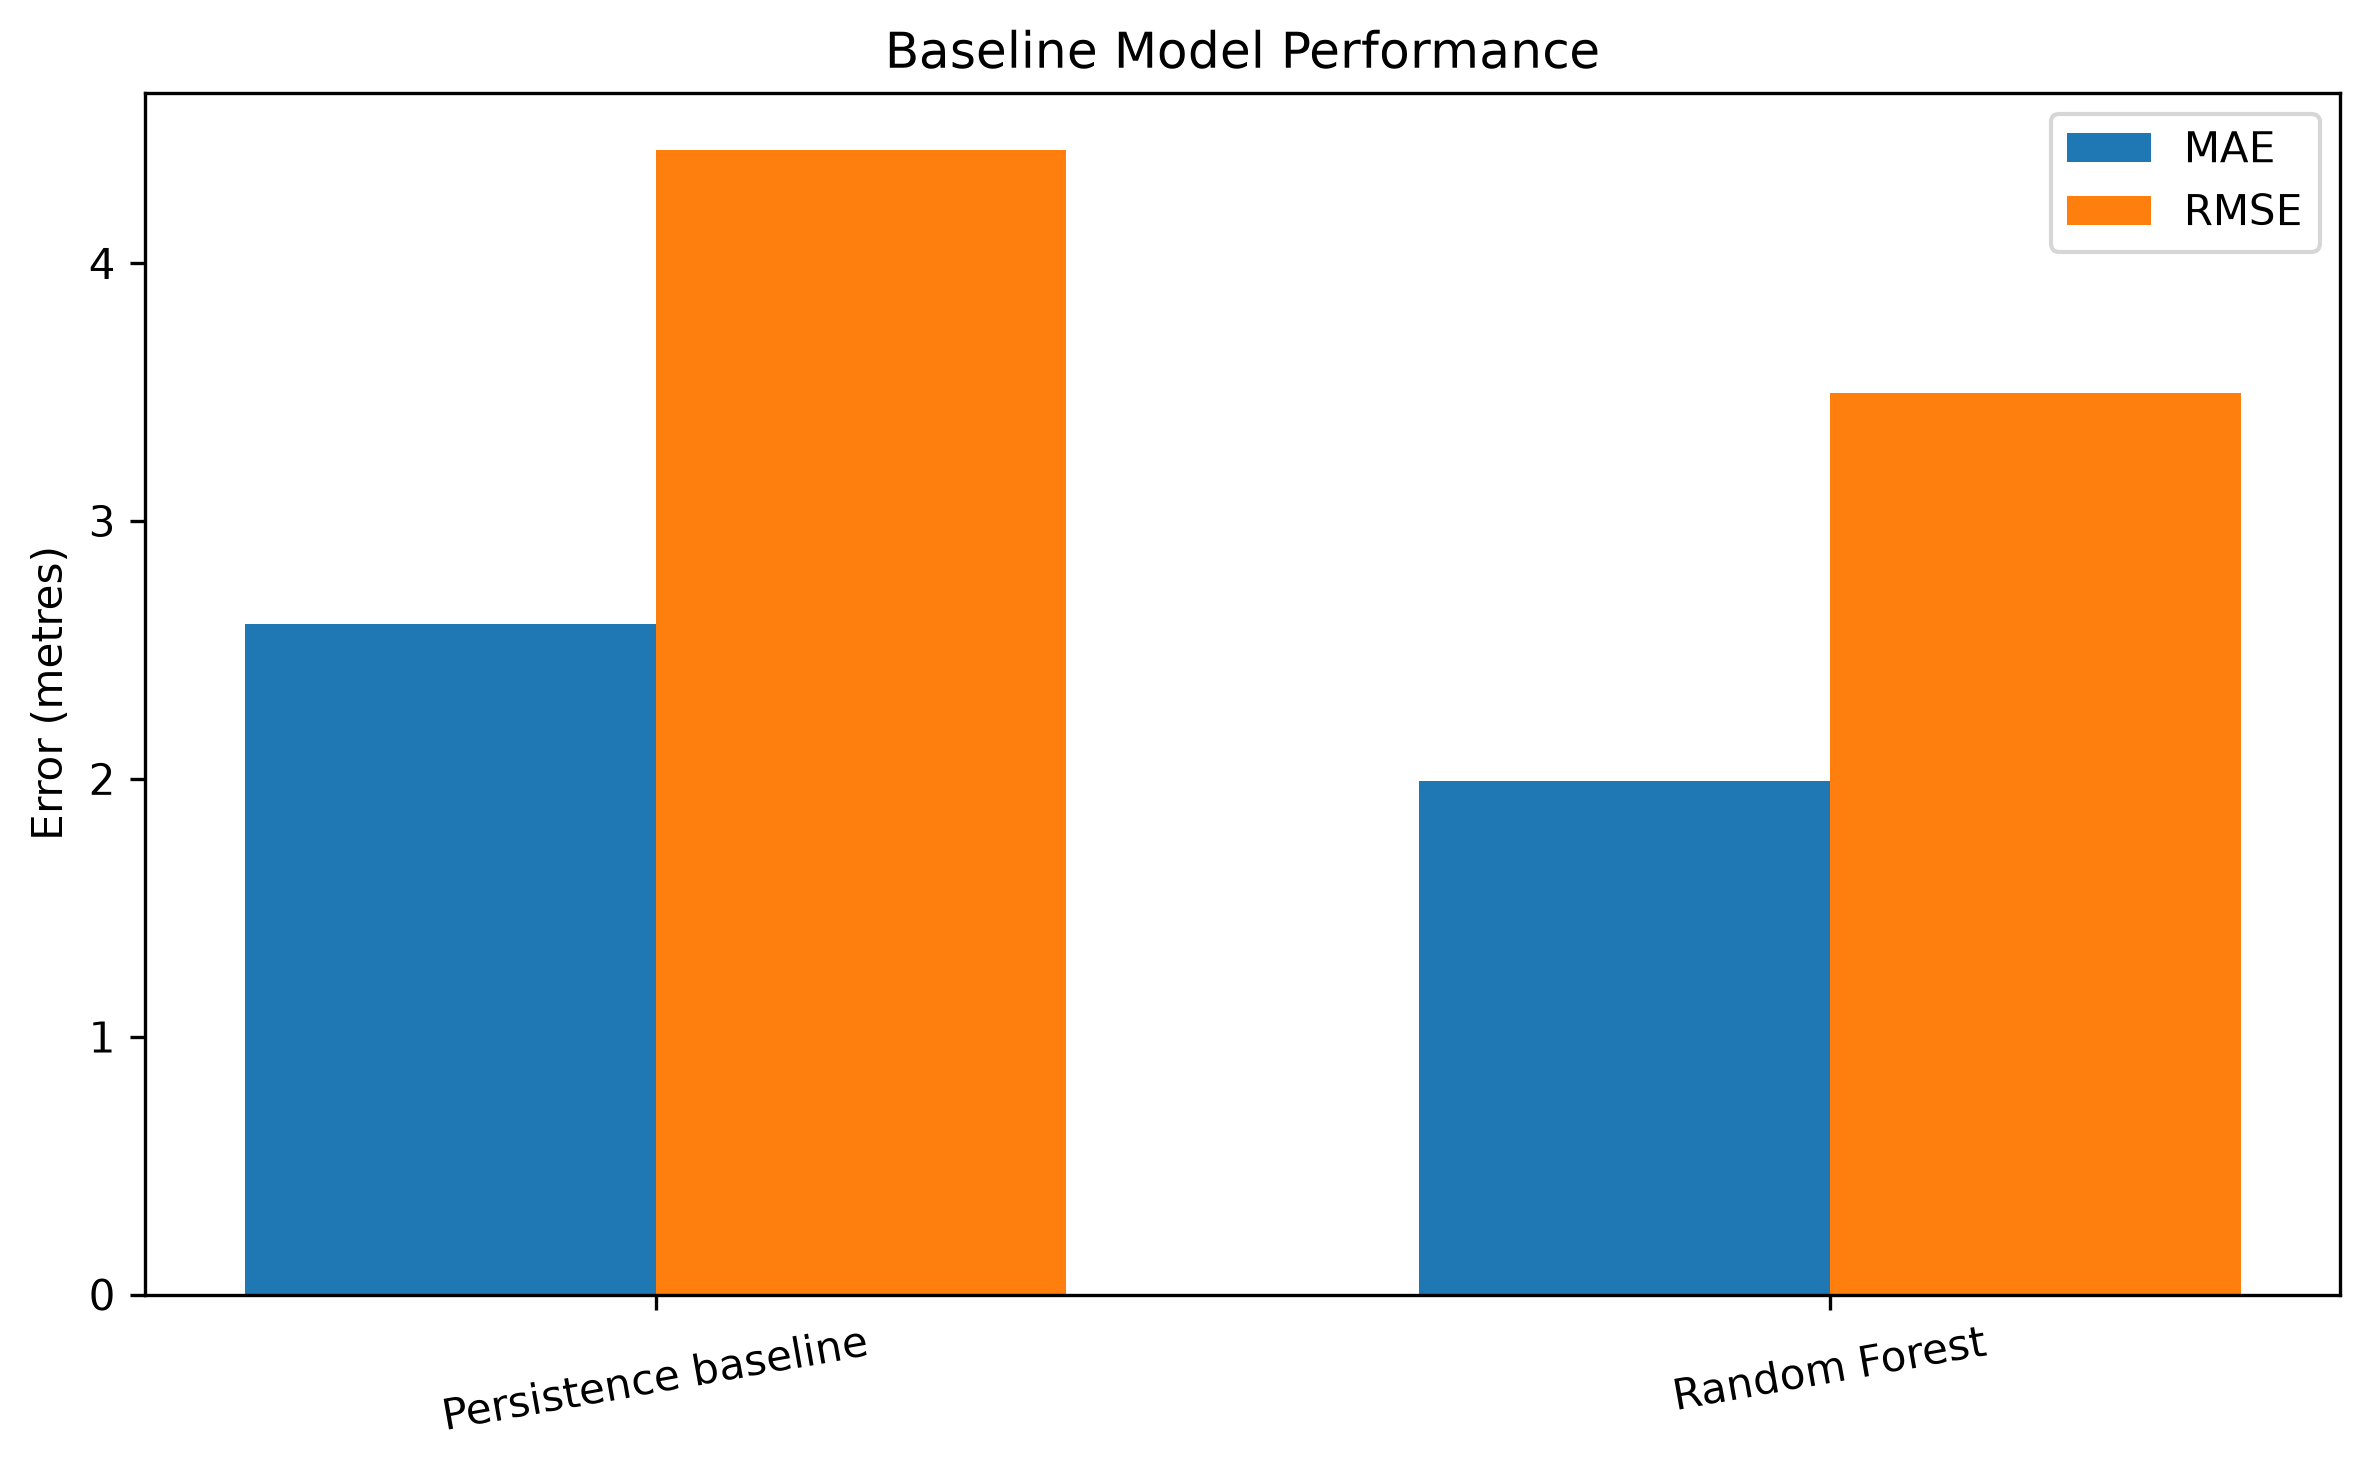
\includegraphics[width=\columnwidth]{figure1_baseline_comparison.png}
  \caption{Comparison of persistence baseline and Random Forest prediction
           errors on the test set. Random Forest reduces MAE by 23.5\,\%
           (from 2.60\,m to 1.99\,m).}
  \label{fig:baseline}
\end{figure}

\subsection{Input Extrapolation — Full-Feature Novelty}

Table~\ref{tab:novelty_full} presents prediction errors stratified by
novelty group for full seven-feature novelty.
MAE increases from 1.82\,m in the familiar group to 3.34\,m in the
extreme-novelty group, an increase of 83.9\,\%.
The well-level bootstrap CIs for group MAE differences exclude zero,
indicating statistically conclusive differences between groups.
Figure~\ref{fig:novelty} illustrates the error increase across novelty
groups.

\begin{table}[htbp]
\centering
\caption{Full-Feature Novelty: Prediction Errors by Group
         (95th-pctile threshold = 0.350; 99th-pctile = 0.554)}
\label{tab:novelty_full}
\begin{tabular}{@{}lrrrr@{}}
\toprule
\textbf{Group} & \textbf{N\,obs} & \textbf{N\,wells} & \textbf{MAE (m)} & \textbf{RMSE (m)} \\
\midrule
Familiar          & 13{,}082 & 1{,}768 & 1.8155 & 2.9295 \\
Poorly represented &  1{,}090 &   674   & 3.2271 & 6.0301 \\
Extreme novelty   &     691   &   503   & 3.3383 & 6.5833 \\
\bottomrule
\end{tabular}
\end{table}

\begin{figure}[htbp]
  \centering
  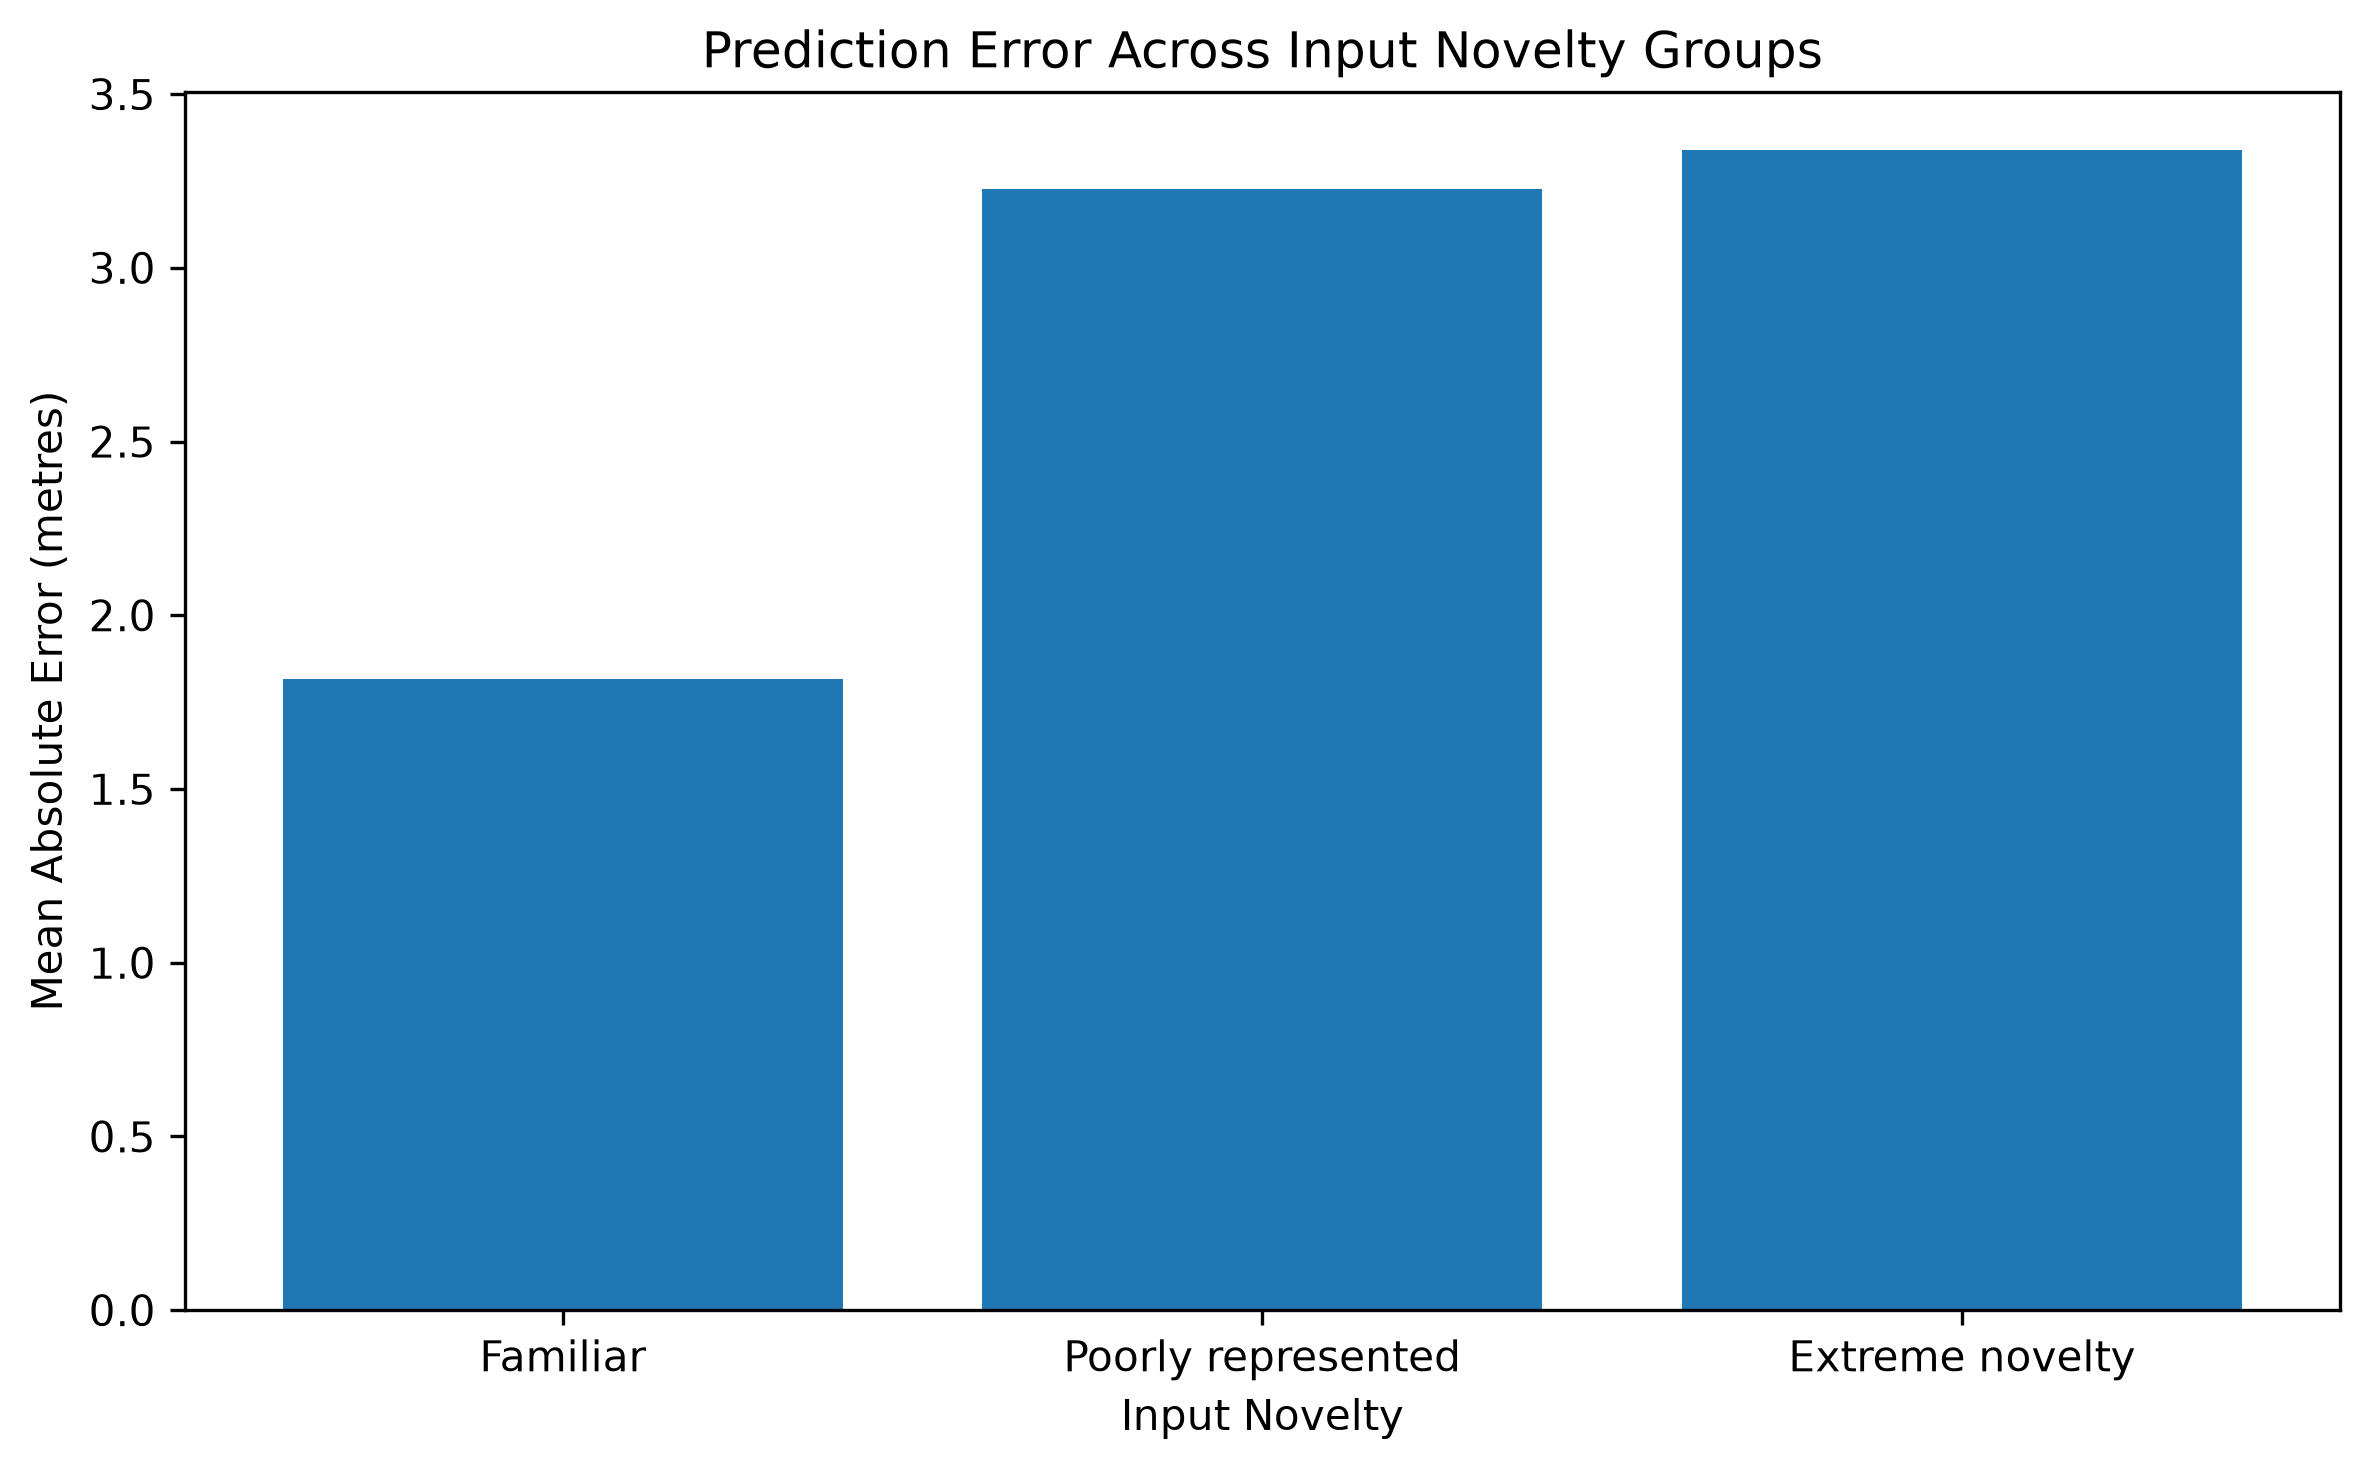
\includegraphics[width=\columnwidth]{figure2_input_novelty.png}
  \caption{Prediction MAE across full-feature novelty groups.
           Error bars represent well-level bootstrap 95\,\% CIs.
           Both poorly-represented and extreme-novelty groups show
           substantially higher errors than familiar observations.}
  \label{fig:novelty}
\end{figure}

\subsection{Rainfall-Only Novelty}

Table~\ref{tab:novelty_rain} shows that when novelty is computed using
only the two rainfall features, the monotonic error increase disappears.
The extreme-novelty group has lower MAE (1.82\,m) than the
poorly-represented group (2.27\,m) and similar MAE to the familiar
group (1.93\,m).
This finding is important: the full-feature novelty effect cannot be
attributed to rainfall novelty alone.

\begin{table}[htbp]
\centering
\caption{Rainfall-Only Novelty: Prediction Errors by Group
         (95th-pctile threshold = 0.0073; 99th-pctile = 0.0500)}
\label{tab:novelty_rain}
\begin{tabular}{@{}lrrrr@{}}
\toprule
\textbf{Group} & \textbf{N\,obs} & \textbf{N\,wells} & \textbf{MAE (m)} & \textbf{RMSE (m)} \\
\midrule
Familiar           & 10{,}684 & 1{,}773 & 1.9311 & 3.4819 \\
Poorly represented &  2{,}962 & 1{,}420 & 2.2731 & 3.9050 \\
Extreme novelty    &  1{,}217 &   509   & 1.8153 & 2.4250 \\
\bottomrule
\end{tabular}
\end{table}

\subsection{Novelty Type Comparison}

Table~\ref{tab:novelty_type} compares the lowest (Q1) and highest (Q4)
novelty quartiles for geographic, environmental, and combined novelty
definitions.
Geographic novelty produces essentially flat MAE across quartiles
(Q1: 1.90\,m, Q4: 1.91\,m), while environmental novelty shows a 78.8\,\%
increase (Q1: 1.54\,m, Q4: 2.75\,m) and combined novelty a 107.3\,\%
increase (Q1: 1.39\,m, Q4: 2.87\,m).
Figure~\ref{fig:novelty_types} illustrates these patterns.

\begin{table}[htbp]
\centering
\caption{Novelty Type Comparison: MAE in Q1 and Q4 Quartiles
         (approx.\ 3,715--3,716 observations per quartile)}
\label{tab:novelty_type}
\begin{tabular}{@{}lrrr@{}}
\toprule
\textbf{Novelty Type} & \textbf{Q1 MAE (m)} & \textbf{Q4 MAE (m)} & \textbf{Increase} \\
\midrule
Geographic   & 1.9015 & 1.9054 &  +0.2\,\% \\
Environmental & 1.5406 & 2.7542 & +78.8\,\% \\
Combined      & 1.3864 & 2.8737 & +107.3\,\% \\
\bottomrule
\end{tabular}
\end{table}

\begin{figure}[htbp]
  \centering
  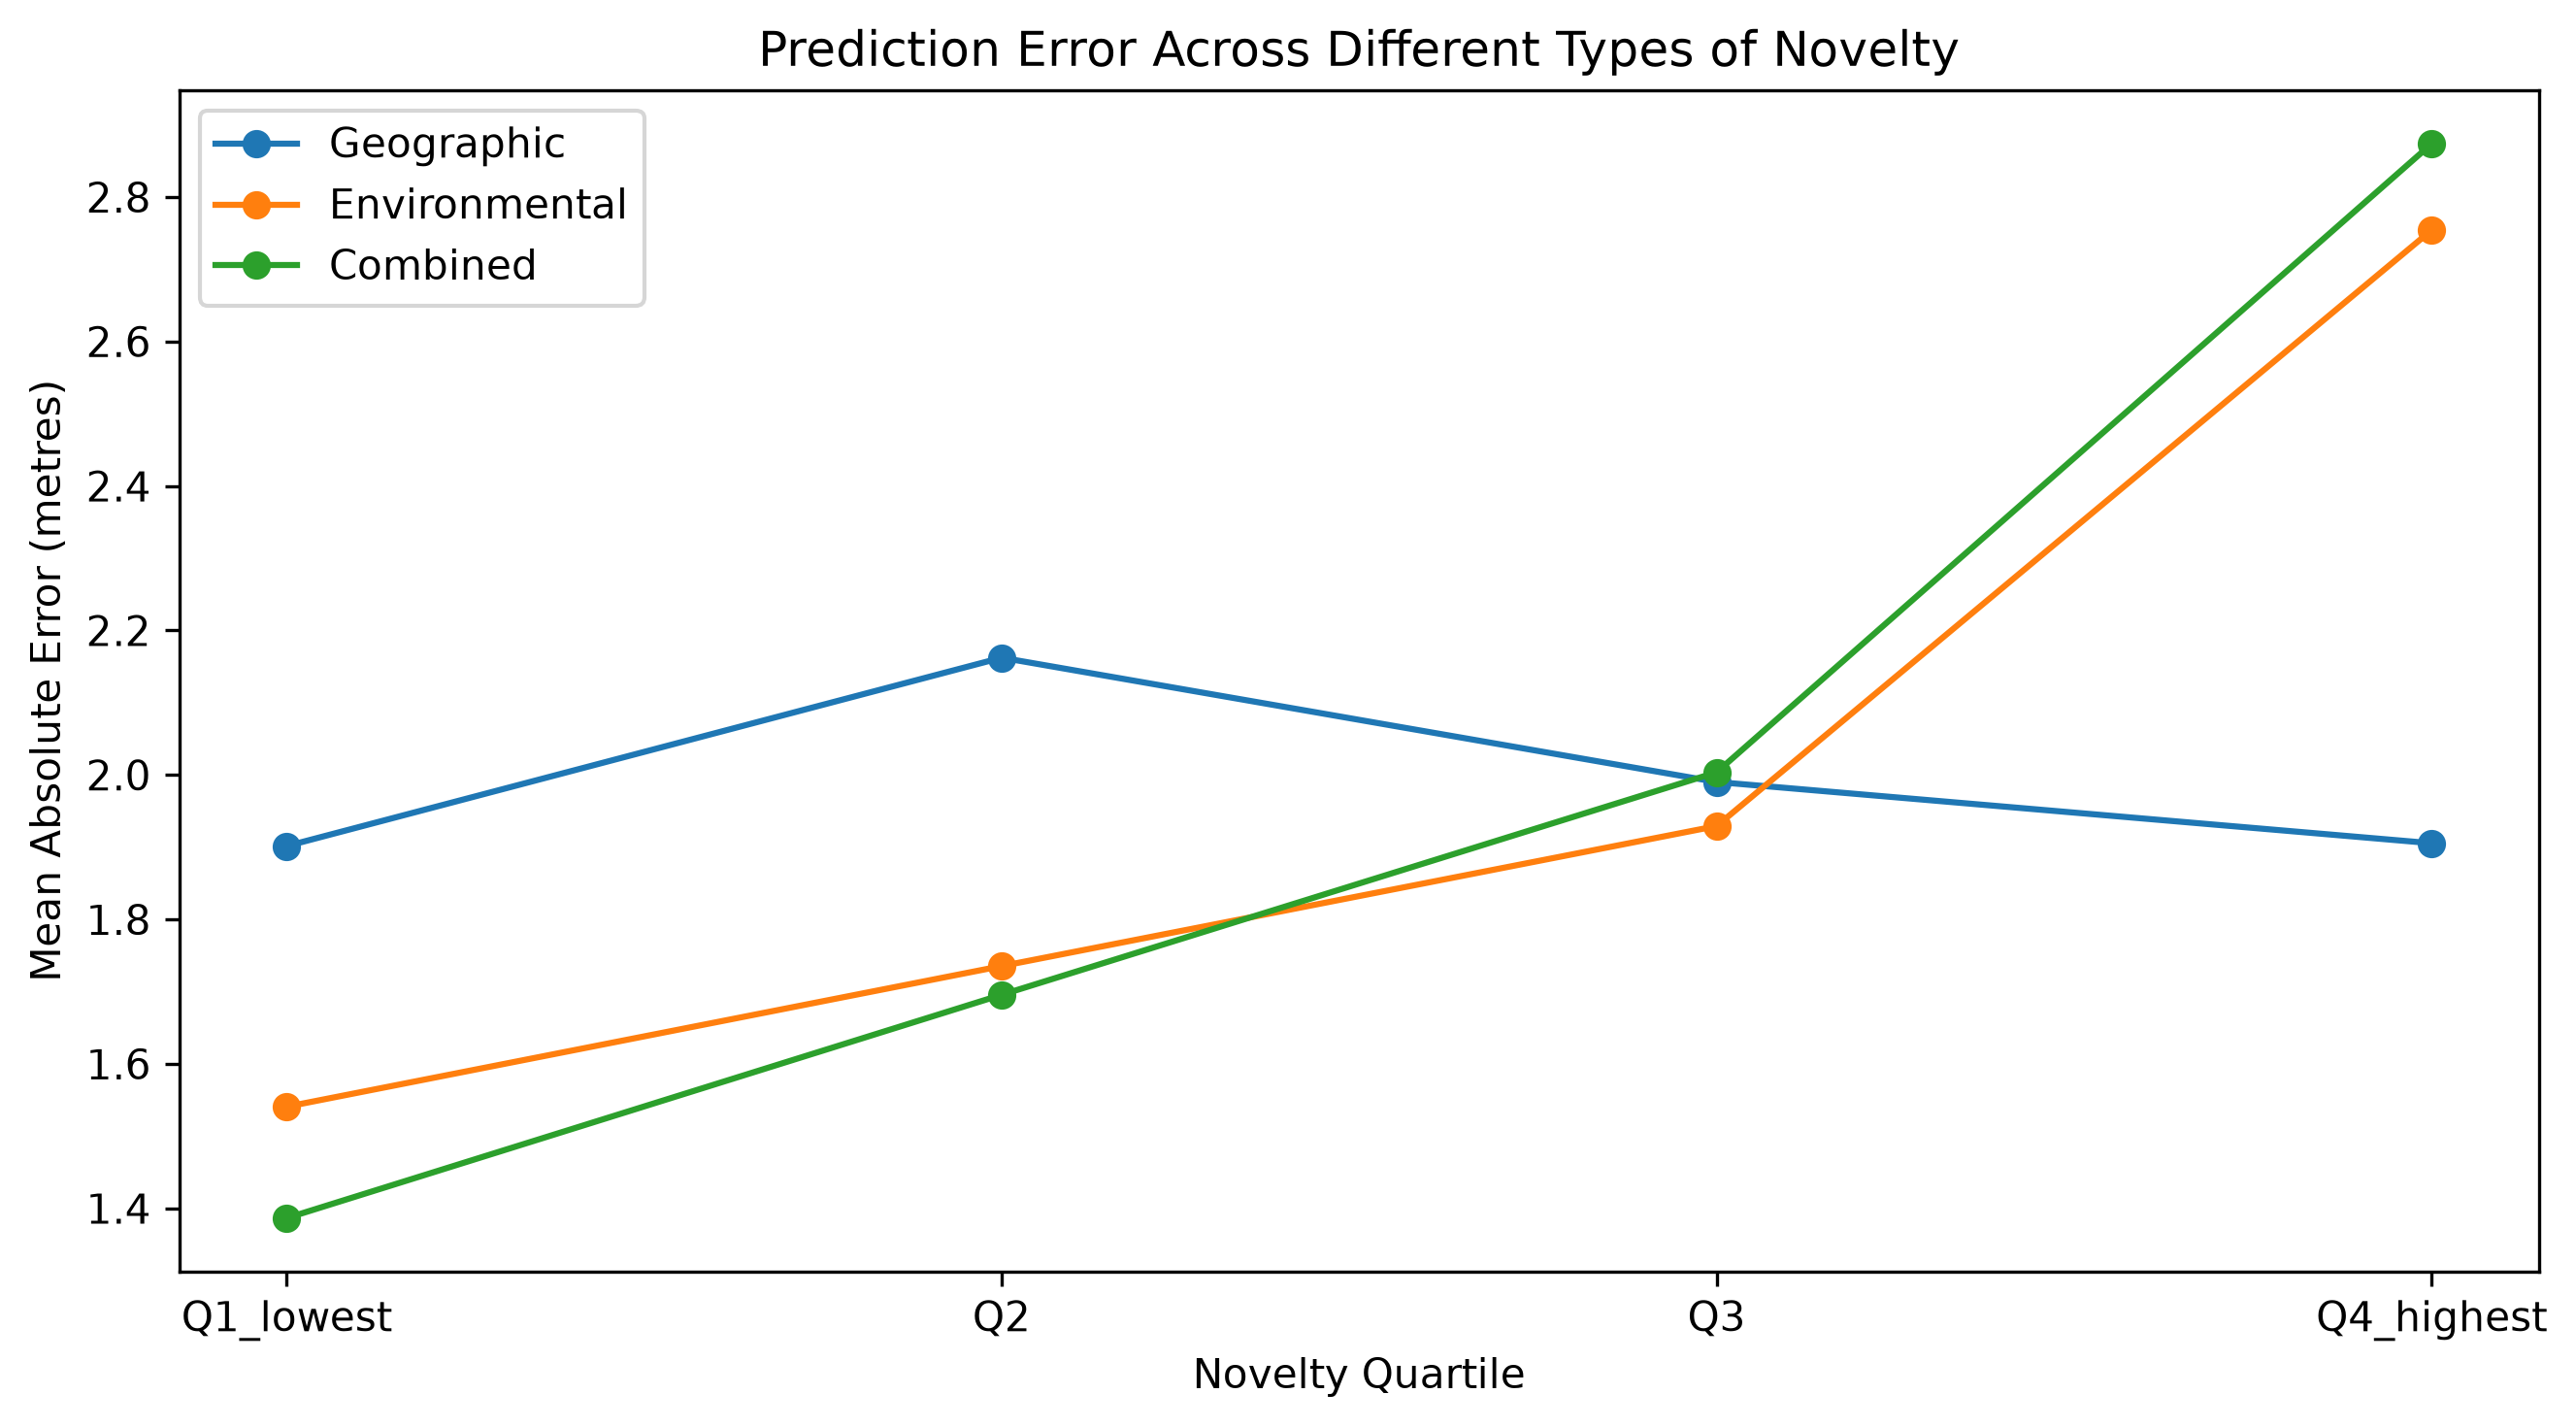
\includegraphics[width=\columnwidth]{figure3_novelty_types.png}
  \caption{MAE by novelty quartile for geographic, environmental,
           and combined feature-space novelty. Environmental and combined
           novelty show strong error increases in the highest quartile;
           geographic novelty does not.}
  \label{fig:novelty_types}
\end{figure}

\subsection{Person 3 Grouped Evaluation}

Table~\ref{tab:p3_grouped} reports Person 3's grouped evaluation using
training-derived rainfall bounds.
Under both the 5th--95th and 1st--99th percentile definitions, unfamiliar
observations have \emph{lower} MAE than familiar ones.
This counter-intuitive direction is explained by a between-well confound
(Section~\ref{sec:discussion}).

\begin{table}[htbp]
\centering
\caption{Person 3 Grouped Evaluation: Familiar vs.\ Unfamiliar Rainfall
         (thresholds from training data only)}
\label{tab:p3_grouped}
\begin{tabular}{@{}lrrrr@{}}
\toprule
\textbf{Group} & \textbf{N\,obs} & \textbf{N\,wells} & \textbf{MAE (m)} & \textbf{RMSE (m)} \\
\midrule
Familiar (5th--95th)   & 13{,}133 & 1{,}792 & 2.0011 & 3.5312 \\
Unfamiliar (5th--95th) &  1{,}730 &   827   & 1.9062 & 3.2318 \\
Familiar (1st--99th)   & 14{,}314 & 1{,}795 & 2.0048 & 3.5420 \\
Unfamiliar (1st--99th) &    549   &   353   & 1.6053 & 2.0238 \\
Below 95th pctile (rain) & 13{,}758 & 1{,}793 & 2.0164 & 3.5846 \\
High rainfall ($\geq$95th pctile) & 1{,}105 & 388 & 1.6625 & 2.1383 \\
\bottomrule
\end{tabular}
\end{table}

\subsection{Bootstrap Confidence Intervals}

Table~\ref{tab:bootstrap} reports the key bootstrap CIs from Person 3's
verification.
The RF vs.\ persistence CI excludes zero, confirming the baseline
improvement.
The corrected within-well unfamiliar--familiar CI ($+0.186$\,m,
$[+0.068, +0.307]$) excludes zero, suggesting that within wells with
observations in both familiar and unfamiliar conditions, unfamiliar
observations are associated with higher errors.
The same-well high-rainfall CI ($-0.041$\,m, $[-0.169, +0.080]$) includes
zero, indicating no conclusive within-well high-rainfall effect.

\begin{table}[htbp]
\centering
\caption{Bootstrap 95\,\% Confidence Intervals (Well-Level Cluster,
         $B = 2{,}000$ Repetitions)}
\label{tab:bootstrap}
\begin{tabular}{@{}p{4.2cm}rrr@{}}
\toprule
\textbf{Quantity} & \textbf{Point (m)} & \textbf{95\,\% CI (m)} & \textbf{Excl.\ 0?} \\
\midrule
RF $-$ Persistence MAE        & $-0.636$ & $[-0.728, -0.562]$ & Yes \\
Unfam.$-$Fam.\ MAE (corrected paired) & $+0.186$ & $[+0.068, +0.307]$ & Yes \\
High-rain $-$ Normal MAE (unpaired) & $-0.549$ & $[-0.715, -0.384]$ & Yes \\
Same-well paired MAE diff.     & $-0.041$ & $[-0.169, +0.080]$ & No \\
\bottomrule
\end{tabular}
\end{table}

\begin{figure}[htbp]
  \centering
  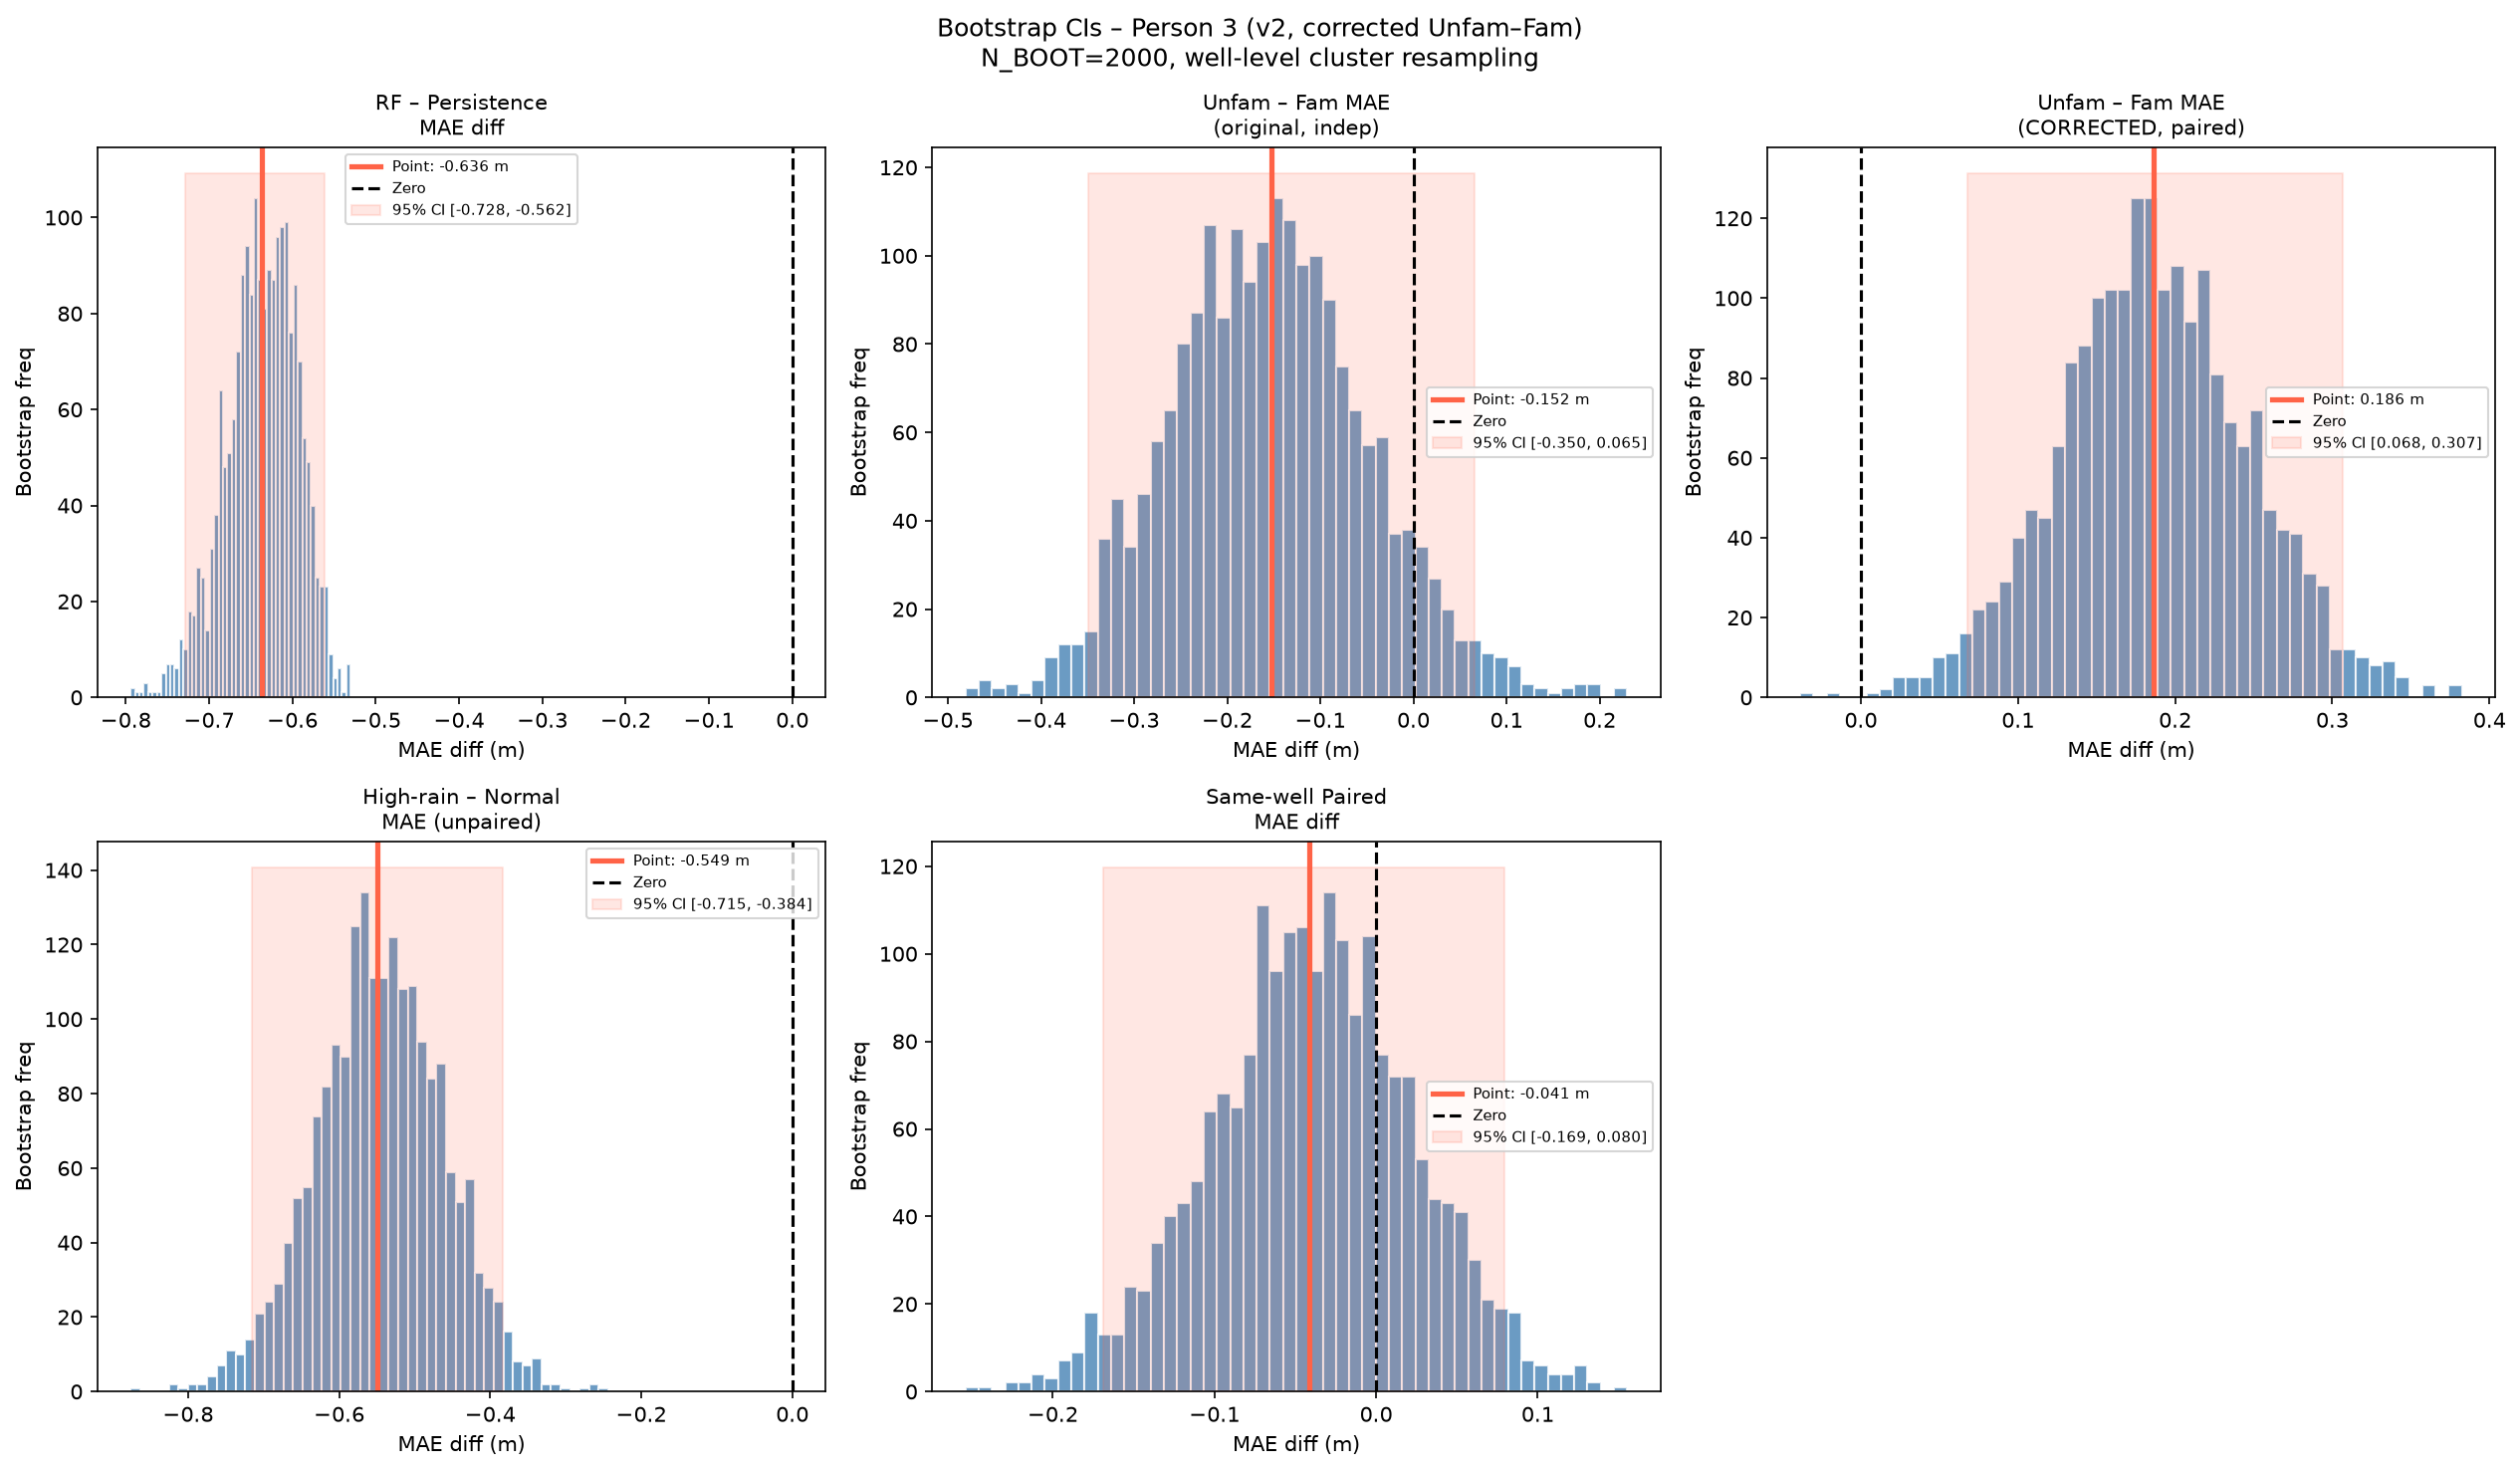
\includegraphics[width=\columnwidth]{bootstrap_results.png}
  \caption{Bootstrap 95\,\% confidence intervals for key comparisons.
           The corrected within-well unfamiliar--familiar CI excludes zero;
           the same-well high-rainfall CI does not.}
  \label{fig:bootstrap}
\end{figure}

\subsection{Same-Well Evaluation}

Table~\ref{tab:same_well} reports the within-well high-rainfall vs.\
normal comparison.
Across 386 eligible wells, the mean paired difference is $-0.041$\,m with
a CI $[-0.168, +0.080]$ that includes zero.
Approximately 49\,\% of wells show higher error under high-rainfall
conditions, consistent with no systematic within-well effect.

\begin{table}[htbp]
\centering
\caption{Same-Well Paired Evaluation: High-Rainfall vs.\ Normal
         (386 Eligible Wells, $B = 2{,}000$ Bootstrap Reps)}
\label{tab:same_well}
\begin{tabular}{@{}lr@{}}
\toprule
\textbf{Metric} & \textbf{Value} \\
\midrule
Eligible wells                       & 386 \\
Mean paired diff.\ (high $-$ normal) & $-0.041$\,m \\
Median paired diff.                  & $-0.033$\,m \\
Fraction wells with higher error in high rain & 49.0\,\% \\
Bootstrap 95\,\% CI                  & $[-0.168, +0.080]$\,m \\
CI includes zero                     & Yes \\
\bottomrule
\end{tabular}
\end{table}

\begin{figure}[htbp]
  \centering
  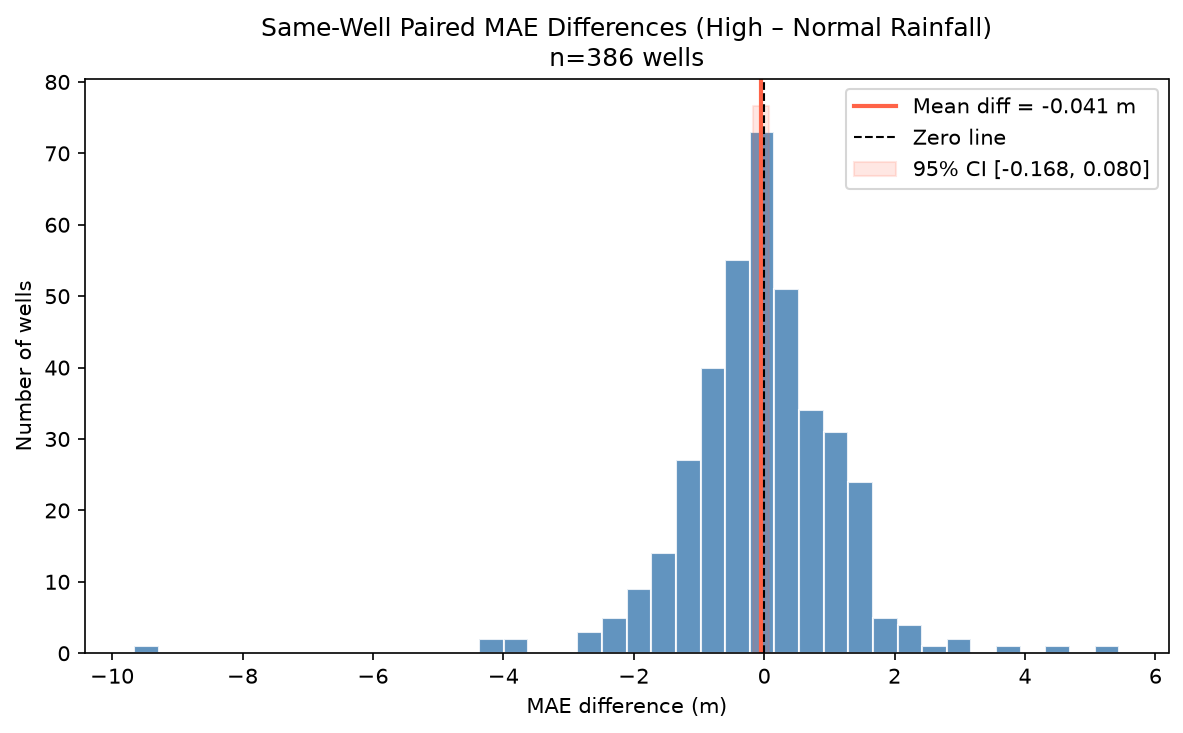
\includegraphics[width=\columnwidth]{same_well_comparison.png}
  \caption{Per-well MAE in normal vs.\ high-rainfall conditions for 386
           eligible wells. The near-diagonal distribution and CI including
           zero indicate no conclusive within-well high-rainfall effect.}
  \label{fig:same_well}
\end{figure}

\subsection{Rainfall QC Sensitivity}

Table~\ref{tab:qc_sensitivity} reports the results of the rainfall
quality-control sensitivity analysis.
Because all eight 30-day and all sixteen 90-day suspicious rainfall flags
fall within the training period, excluding flagged observations leaves the
test-set metrics unchanged.
An additional retrain experiment excluding the 16 flagged training rows
produced a negligible change ($\Delta$MAE $= -0.000$\,m).

\begin{table}[htbp]
\centering
\caption{Rainfall QC Sensitivity Analysis}
\label{tab:qc_sensitivity}
\begin{tabular}{@{}lrrr@{}}
\toprule
\textbf{Scenario} & \textbf{N\,obs} & \textbf{MAE (m)} & \textbf{R\textsuperscript{2}} \\
\midrule
Full test set                       & 14{,}863 & 1.9901 & 0.7690 \\
Excl.\ flag \texttt{qc\_susp\_30d}  & 14{,}863 & 1.9901 & 0.7690 \\
Excl.\ flag \texttt{qc\_susp\_90d}  & 14{,}863 & 1.9901 & 0.7690 \\
\bottomrule
\end{tabular}
\end{table}

\subsection{Controlled Training Removal}

Table~\ref{tab:removal} compares the full, extreme-removed, and
matched-control models.
The overall MAE difference between the extreme-removed and full models
(+0.016\,m, CI $[-0.004, +0.038]$) includes zero.
The clearest deterioration occurs in the poorly-represented group
(+0.082\,m, CI $[+0.031, +0.141]$, excludes zero).
The extreme-novelty group shows a larger estimated change (+0.260\,m) but
with a wide CI ($[-0.150, +0.708]$) that includes zero.

\begin{table}[htbp]
\centering
\caption{Controlled Training Removal: MAE by Model and Test Novelty Group}
\label{tab:removal}
\begin{tabular}{@{}llrr@{}}
\toprule
\textbf{Test group} & \textbf{Model} & \textbf{MAE (m)} & \textbf{R\textsuperscript{2}} \\
\midrule
\multirow{3}{*}{All} & Full           & 1.9898 & 0.7690 \\
                     & Extreme-removed & 2.0061 & 0.7538 \\
                     & Matched-control & 1.9919 & 0.7687 \\
\midrule
\multirow{3}{*}{Familiar} & Full           & 1.8155 & 0.7399 \\
                          & Extreme-removed & 1.8134 & 0.7404 \\
                          & Matched-control & 1.8174 & 0.7398 \\
\midrule
\multirow{3}{*}{Poorly rep.} & Full           & 3.2271 & 0.7624 \\
                             & Extreme-removed & 3.3093 & 0.7407 \\
                             & Matched-control & 3.2278 & 0.7626 \\
\midrule
\multirow{3}{*}{Extreme nov.} & Full           & 3.3383 & 0.8290 \\
                              & Extreme-removed & 3.5985 & 0.7801 \\
                              & Matched-control & 3.3456 & 0.8277 \\
\bottomrule
\end{tabular}
\end{table}

\subsection{Temporal Prediction Error}

Table~\ref{tab:temporal_novelty} presents mean prediction error by year
(derived from \texttt{novelty\_by\_year.csv}).
MAE increases from 1.80\,m in 2018 to 2.29\,m in 2020, a 27.0\,\%
increase over the test period.
The paired temporal comparison (1{,}516 wells) confirms this increase with
a bootstrap CI $[+0.298, +0.531]$\,m excluding zero.
The within-well matched-input comparison (2{,}077 pairs, 1{,}311 wells)
yields a mean error increase of +0.506\,m (CI $[+0.410, +0.605]$\,m),
suggesting that the deterioration persists even when input similarity is
controlled.
Figure~\ref{fig:temporal} displays the temporal error progression.

\begin{table}[htbp]
\centering
\caption{Mean Prediction Error by Test Year (Full-Feature Novelty
         Stratification)}
\label{tab:temporal_novelty}
\begin{tabular}{@{}lrrr@{}}
\toprule
\textbf{Year} & \textbf{N\,obs} & \textbf{Mean novelty} & \textbf{Mean MAE (m)} \\
\midrule
2018 & 6{,}239 & 0.207 & 1.804 \\
2019 & 5{,}629 & 0.243 & 2.035 \\
2020 & 2{,}995 & 0.232 & 2.291 \\
\bottomrule
\end{tabular}
\end{table}

\begin{figure}[htbp]
  \centering
  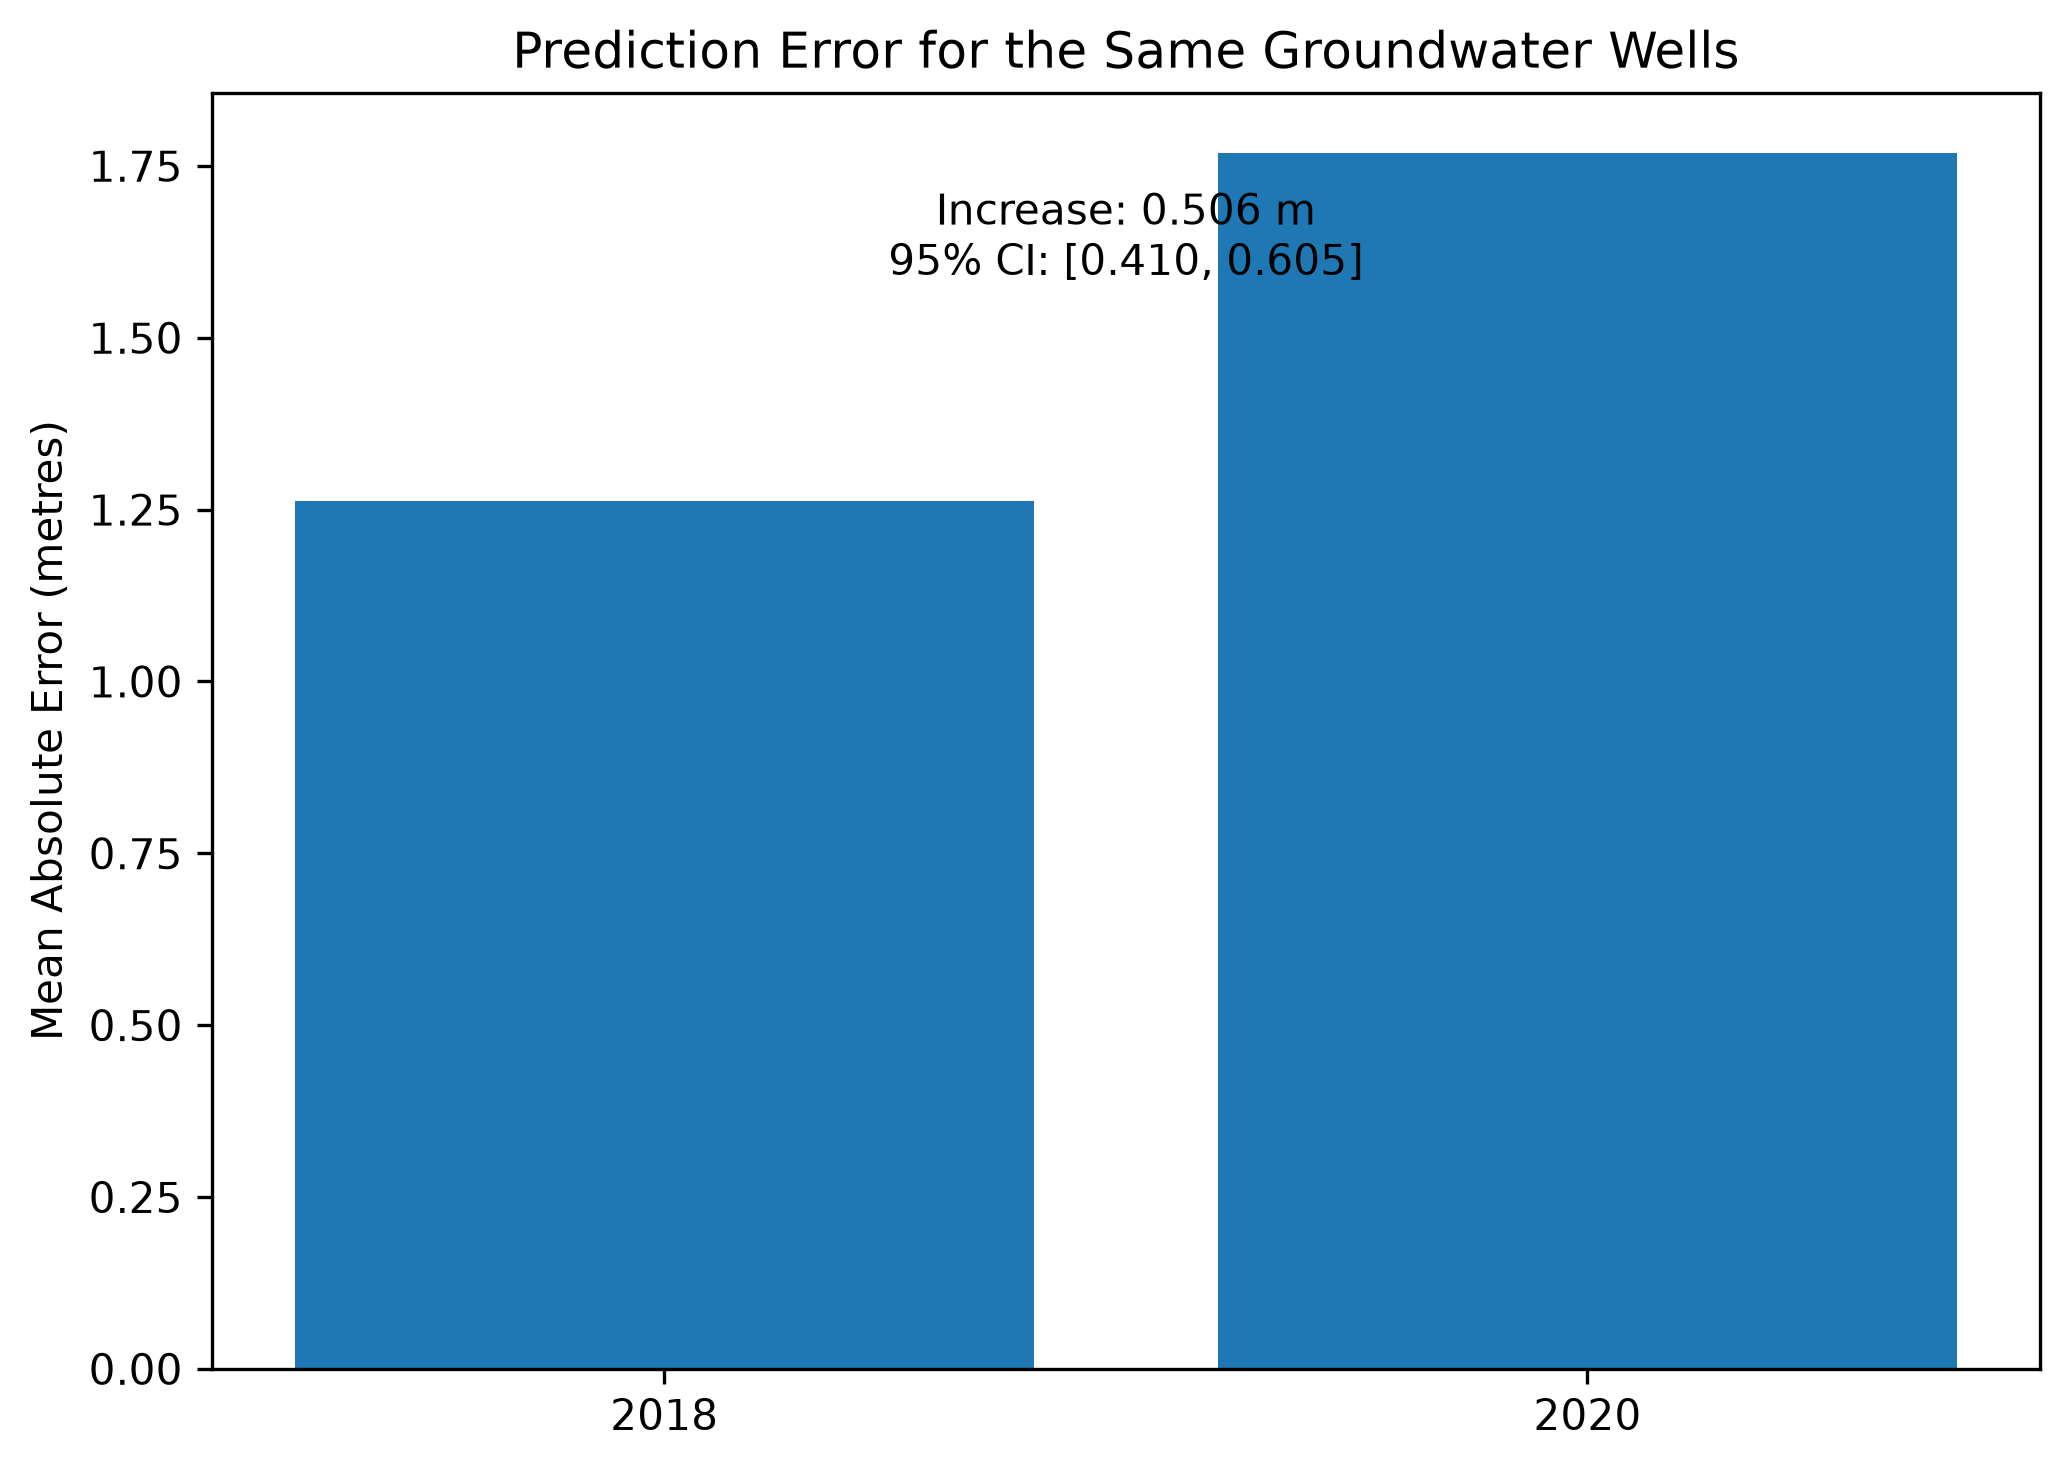
\includegraphics[width=\columnwidth]{figure4_temporal_degradation.png}
  \caption{Temporal evolution of prediction error across the 2018--2020
           test period. MAE increases from 1.80\,m in 2018 to 2.29\,m
           in 2020. Bootstrap CI for the paired 2018--2020 difference
           excludes zero.}
  \label{fig:temporal}
\end{figure}

\subsection{Temporal Residual Regression}

Table~\ref{tab:temporal_reg} reports the residual regression results.
Adding year indicators improves $R^{2}$ slightly (from 0.2727 to 0.2742).
Adding year $\times$ feature interactions increases $R^{2}$ to 0.3044,
indicating that the input--residual relationship changes across years.

\begin{table}[htbp]
\centering
\caption{Temporal Residual Regression: Within-Well Demeaned OLS
         (n = 12,142 observations, 1,479 wells)}
\label{tab:temporal_reg}
\begin{tabular}{@{}lrr@{}}
\toprule
\textbf{Model specification} & \textbf{R\textsuperscript{2}} & \textbf{Adj.\ R\textsuperscript{2}} \\
\midrule
Inputs only                      & 0.2727 & 0.2724 \\
Inputs $+$ year effects          & 0.2742 & 0.2738 \\
Inputs $+$ year $+$ interactions & 0.3044 & 0.3034 \\
\bottomrule
\end{tabular}
\end{table}

\begin{figure}[htbp]
  \centering
  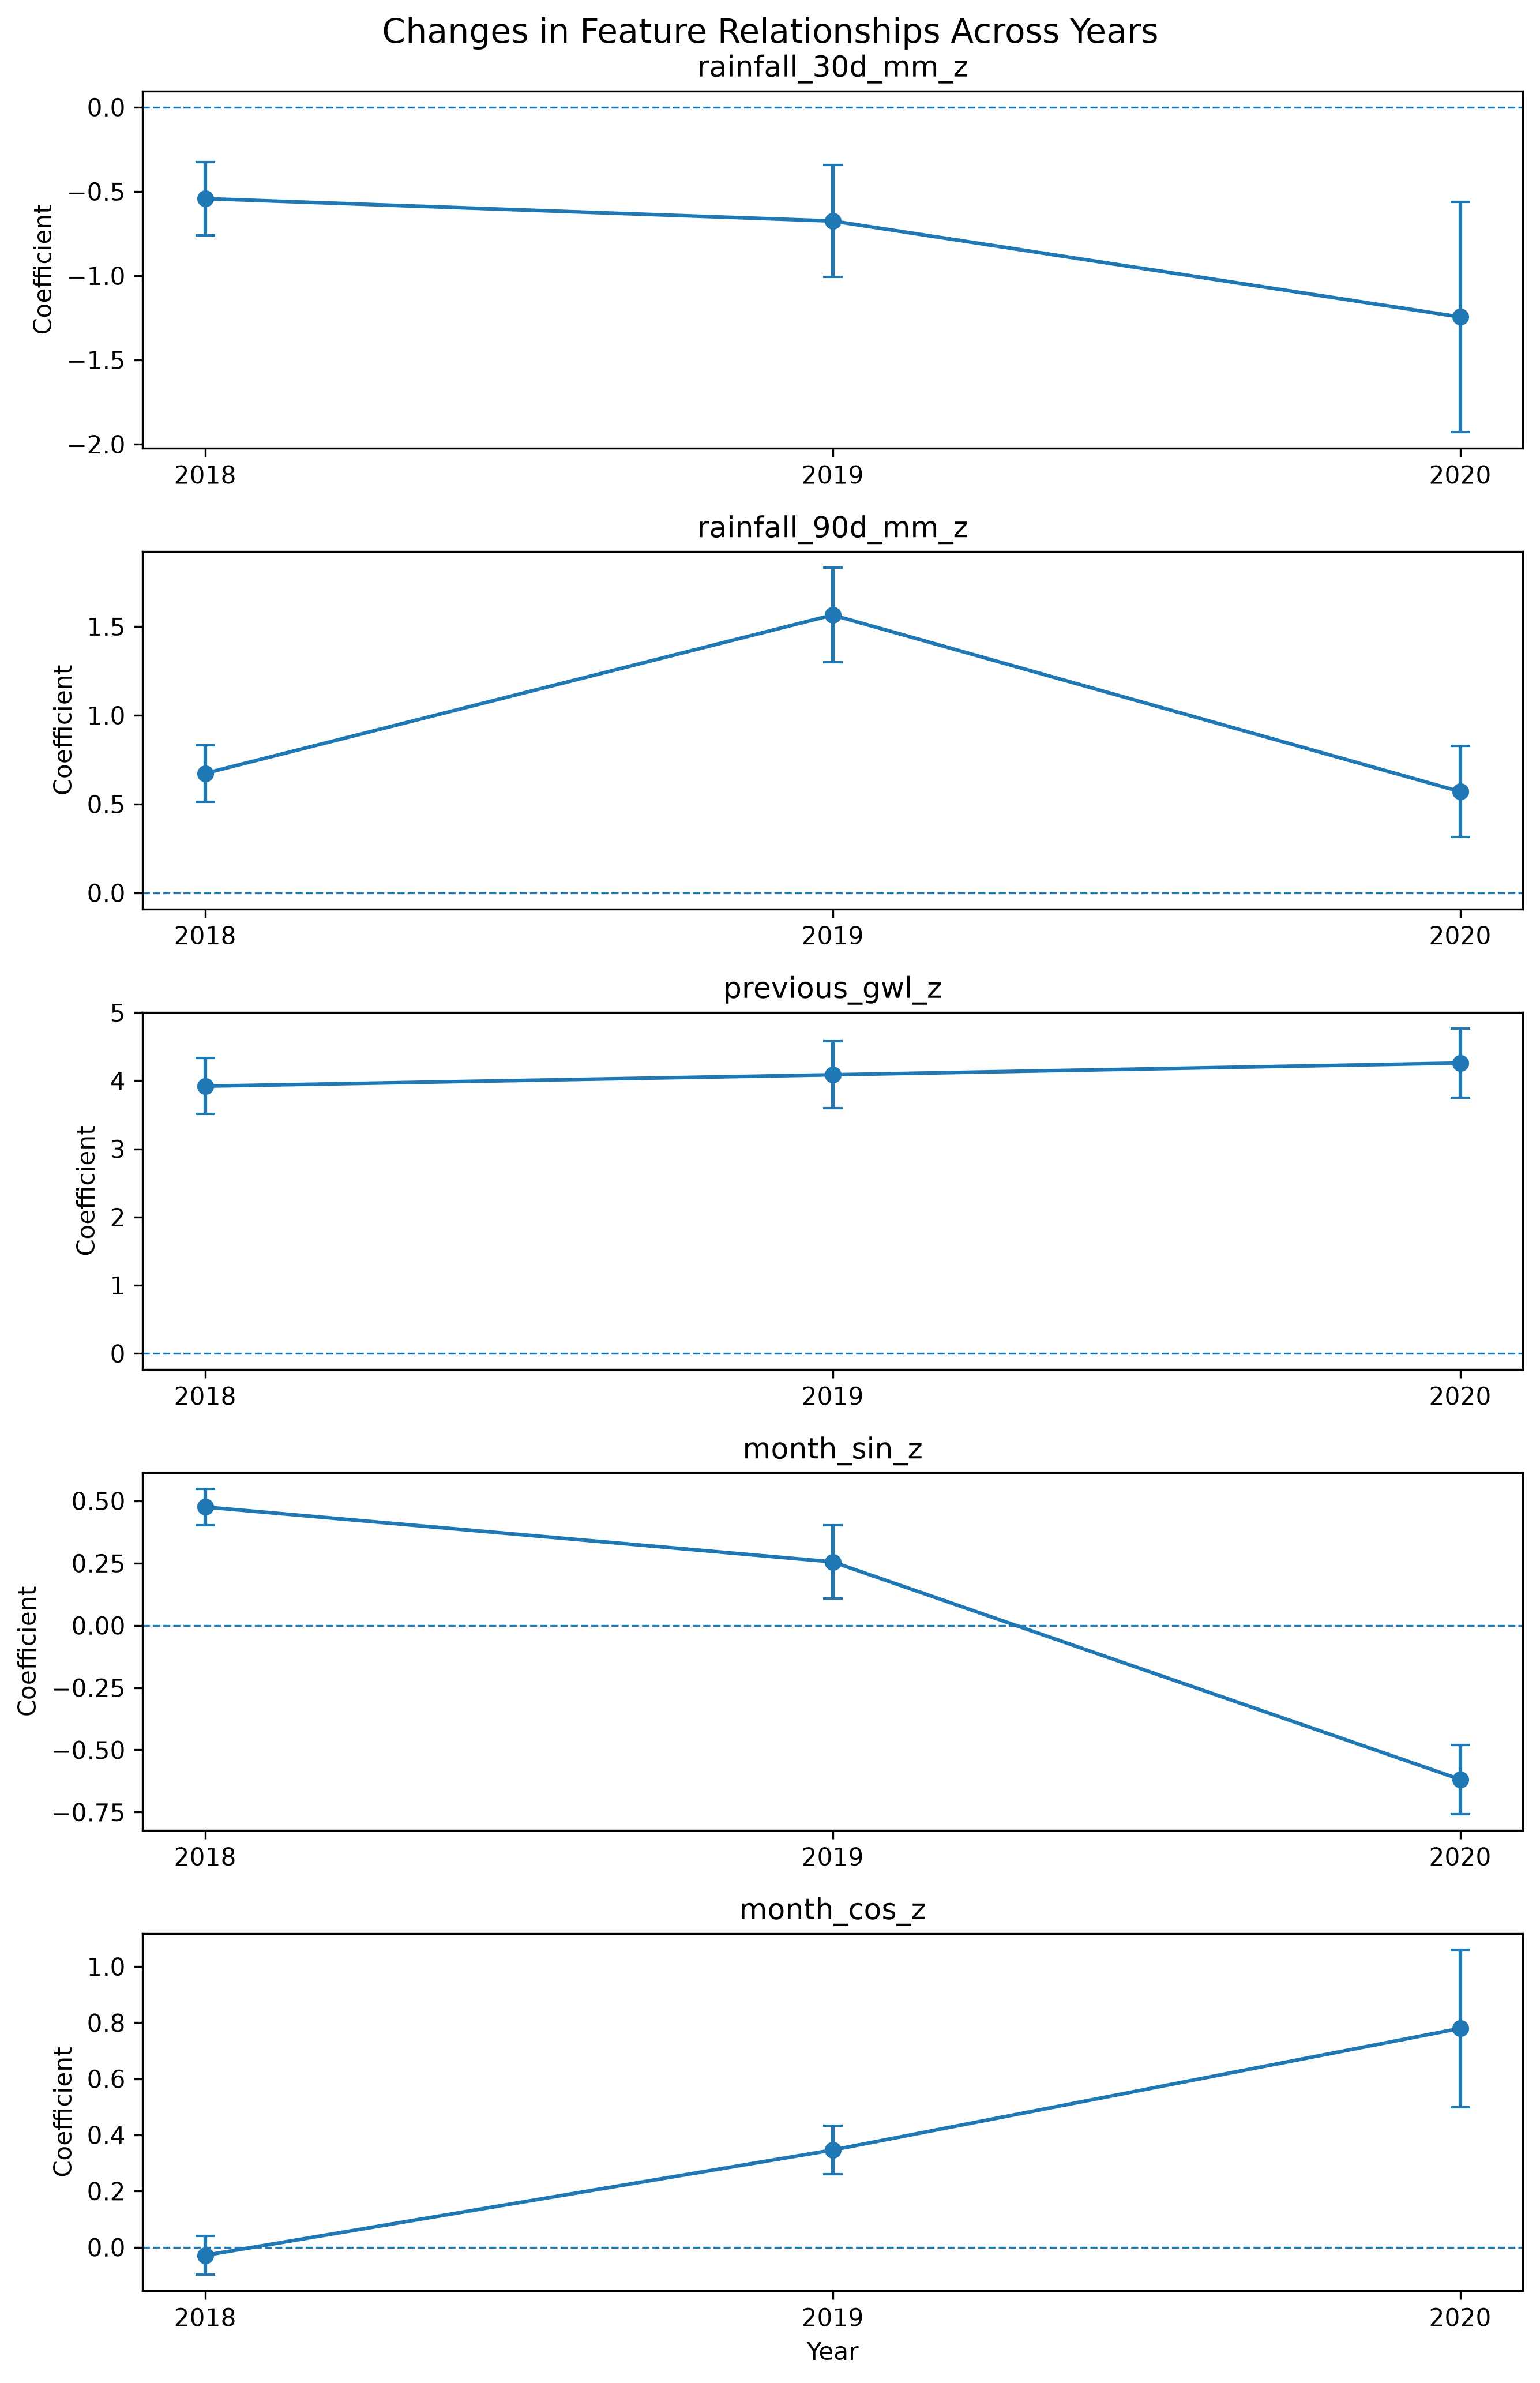
\includegraphics[width=\columnwidth]{figure5_feature_relationships.png}
  \caption{Year-dependent residual regression coefficients for selected
           feature interactions. Interactions involving 90-day rainfall
           and seasonal features are statistically significant, indicating
           that the residual--input relationship changes across years.}
  \label{fig:residuals}
\end{figure}

% ============================================================
\section{Discussion}
\label{sec:discussion}

\subsection{Input Extrapolation as a Source of Error}

The full-feature novelty analysis (Table~\ref{tab:novelty_full}) provides
strong evidence that input extrapolation is associated with higher
prediction errors.
Familiar observations (below the 95th-percentile novelty threshold) have
MAE = 1.82\,m; extreme-novelty observations have MAE = 3.34\,m, an
increase of approximately 1.52\,m (83.9\,\%).
This pattern is robust across different values of $k$, different scalers,
and the Manhattan distance metric (Table in \texttt{results/novelty\_sensitivity.csv}).

However, the rainfall-only novelty analysis (Table~\ref{tab:novelty_rain})
shows \emph{no} monotonic error increase.
Extreme-novelty observations defined using only rainfall features have
\emph{lower} MAE (1.82\,m) than the poorly-represented group (2.27\,m).
This dissociation points to other features---particularly previous GWL,
latitude, and longitude---as important contributors to the full-feature
novelty effect.

The novelty-type comparison (Table~\ref{tab:novelty_type}) reinforces this
interpretation.
Geographic novelty (latitude, longitude) produces essentially flat error
across quartiles, while environmental novelty (rainfall, previous GWL,
seasonal features) and combined novelty both show large error increases in
their upper quartiles.
The combined novelty Q4--Q1 difference is 107.3\,\%, compared to 0.2\,\%
for geographic novelty.
Environmental feature-space novelty is the dominant predictor of elevated
errors; physical distance between wells is not.

\subsection{The Between-Well Confound in Rainfall Comparisons}

Person 3's grouped evaluation (Table~\ref{tab:p3_grouped}) shows that
high-rainfall test observations have \emph{lower} MAE (1.66\,m) than
normal-rainfall observations (2.02\,m).
This appears to contradict the full-feature novelty result, but the
between-well confound identified in Section~\ref{sec:method:p3} explains
the discrepancy.

Of the 1{,}793 wells in the test set, 1{,}407 never experience
high-rainfall observations.
These wells have a substantially higher average MAE (2.38\,m) than the
386 wells that do experience high rainfall (1.73\,m under normal
conditions).
Consequently, the unpaired ``normal'' group contains many
difficult-to-predict wells that simply never see high rainfall.
The same-well paired analysis (Table~\ref{tab:same_well}), which
restricts to the 386 wells with observations in both conditions, yields a
mean difference of only $-0.041$\,m with a CI that includes zero.
This confirms that the apparent high-rainfall advantage is a structural
between-well effect rather than a within-well rainfall benefit.

The corrected within-well unfamiliar--familiar CI
($+0.186$\,m, CI $[+0.068, +0.307]$, Table~\ref{tab:bootstrap}) does
exclude zero, suggesting that within the 824 wells with observations in
both familiar and unfamiliar input conditions, unfamiliar conditions are
associated with somewhat higher errors.
This is a more modest signal than the full-feature novelty result, and
the 95th-percentile rainfall-based unfamiliar definition captures
different observations than the seven-feature distance-based approach.

\subsection{Temporal Predictive Relationship Instability}

Temporal prediction errors increase substantially across the test period
(Table~\ref{tab:temporal_novelty}).
The paired temporal analysis (1{,}516 wells) and within-well matched-input
comparison (2{,}077 pairs) both yield bootstrap CIs that exclude zero,
indicating statistically conclusive deterioration.

Critically, the matched-input comparison controls for input similarity
within wells: observations from 2018 and 2020 are paired by their values
of rainfall, previous GWL, and seasonal features, yet 2020 errors remain
0.51\,m higher on average.
This residual deterioration suggests that the learned input--output
relationship may have changed between the training period and 2020 in a
way not fully captured by the input features used.

The temporal residual regression (Table~\ref{tab:temporal_reg}) provides
further evidence.
The improvement in $R^{2}$ from 0.2727 (inputs only) to 0.3044
(inputs $+$ year $\times$ feature interactions) indicates that the
year-conditional input--residual relationship accounts for additional
variation.
Several year $\times$ feature interactions are statistically significant:
for example, the 2019 $\times$ 90-day rainfall coefficient is $+0.892$
($p = 8.19 \times 10^{-13}$) and the 2020 $\times$ month cosine
coefficient is $+0.808$ ($p = 3.10 \times 10^{-8}$).
These are residual regression associations, not direct estimates of the
Random Forest's learned feature weights, and must be interpreted
accordingly.

The controlled training-removal experiment (Table~\ref{tab:removal})
shows that removing the top 1\,\% most novel training observations
increases MAE in the poorly-represented group by $+0.082$\,m
(CI $[+0.031, +0.141]$, excludes zero).
The overall and extreme-novelty group CIs include zero, indicating that
the aggregate impact is not statistically conclusive at this removal scale.
The result is consistent with training data coverage being one contributor
to the novelty--error association.

\subsection{Practical Implications}

These findings have several practical implications.
First, groundwater ML models should be evaluated not only on overall
held-out metrics but also on the subset of observations that fall outside
the training feature-space coverage.
Near-neighbour novelty scores are computationally inexpensive and can be
computed at deployment time to flag predictions that may be unreliable.

Second, environmental feature-space novelty (driven by unusual
combinations of rainfall, prior GWL, and seasonality) is a better
predictor of prediction quality than geographic distance.
Monitoring networks and training data collection should prioritise
environmental coverage rather than spatial spread alone.

Third, the evidence of temporal deterioration in matched-input comparisons
suggests that static models trained on historical data may require
periodic retraining as groundwater dynamics evolve.
The absence of prediction intervals (Person 2 gap) leaves the question of
calibrated uncertainty quantification open for future work.

% ============================================================
\section{Limitations}
\label{sec:limitations}

\begin{enumerate}
  \item \textbf{Rolling one-step-ahead setting.} The use of
        \texttt{previous\_gwl} as a feature assumes that the previous
        observation is available at prediction time.
        This is not equivalent to a fixed-origin multi-step forecast.

  \item \textbf{Novelty as feature-space distance.} The nearest-neighbour
        novelty score measures distance in input space; it does not
        identify physical extreme events (floods, droughts) directly.
        An observation can be in the extreme-novelty group without
        corresponding to a physically anomalous event.

  \item \textbf{Environmental $\neq$ rainfall-only novelty.}
        Environmental novelty includes previous GWL and seasonal
        features in addition to rainfall; it must not be equated with
        high-rainfall novelty.

  \item \textbf{Different eligibility criteria across experiments.}
        The input-novelty, temporal-pairing, matched-input, and
        within-well analyses use different observation and well
        eligibility criteria.
        Their sample counts are not interchangeable.

  \item \textbf{Control-matching by year only.} In the controlled
        training-removal experiment, control observations are matched
        by year but not by well or environmental characteristics.

  \item \textbf{Temporal distribution changes.} Groundwater levels, 30-day
        rainfall, and 90-day rainfall differ across 2018, 2019, and 2020
        (see research handoff, Section 9).
        Temporal comparisons may confound input-distribution changes with
        genuine relationship instability.

  \item \textbf{Residual regression interpretation.} Temporal interaction
        coefficients describe associations in model residuals, not direct
        changes in the Random Forest's learned feature effects.

  \item \textbf{Potential measurement effects.} Changes in measurement
        procedures, observation quality, and unobserved variables
        (groundwater extraction, irrigation, land use) may contribute to
        temporal differences.

  \item \textbf{Rainfall rolling-window convention.} The Person 3 audit
        confirms that the rainfall QC sensitivity analysis performs an
        evaluation filter only, not a model retrain.
        Because all suspicious flags are in the training period, both
        produce identical test metrics here, but the distinction is
        important for general applicability.

  \item \textbf{Absent Person 2 reliability modelling.} Prediction interval
        coverage, conformal calibration, and interval width analysis
        cannot be evaluated because the corresponding outputs
        (\texttt{reliability\_metrics.csv},
        \texttt{reliability\_predictions.csv},
        \texttt{reliability\_by\_condition.csv},
        \texttt{reliability\_sensitivity.csv})
        are absent from the repository.

  \item \textbf{Bootstrap cross-group independence.} Wells appearing in
        both familiar and unfamiliar groups slightly violate the
        independence assumption of the cross-group bootstrap, leading to
        a small underestimation of CI width.
        The corrected paired bootstrap (Section~\ref{sec:method:p3})
        addresses this.

  \item \textbf{Small high-rainfall sample per well.}
        The median number of high-rainfall observations per eligible well
        is 2, making per-well mean estimates unreliable.

  \item \textbf{Generalisability.} This study uses a single dataset from
        Karnataka, India, with a single chronological split.
        Results may not generalise to other regions, aquifer types, or
        split strategies.
\end{enumerate}

% ============================================================
\section{Conclusion and Future Work}
\label{sec:conclusion}

This paper investigated why a Random Forest groundwater level model
performs poorly under extreme hydroclimatic conditions, separating the
contributions of input extrapolation and predictive relationship
instability.

Using 102{,}289 observations from Karnataka, India, with a chronological
2018 split, we found that:

\begin{itemize}
  \item The Random Forest reduces MAE by 23.5\,\% over the persistence
        baseline (2.60\,m $\rightarrow$ 1.99\,m).
  \item Full-feature novelty is strongly associated with higher prediction
        errors (MAE 1.82\,m at familiar $\rightarrow$ 3.34\,m at extreme
        novelty, $+$83.9\,\%).
  \item Environmental novelty (rainfall, previous GWL, seasonal features)
        explains the error increase; geographic distance alone does not.
  \item Rainfall-only novelty does not produce a monotonic error increase,
        indicating that rainfall extremity alone is insufficient to explain
        the full-feature effect.
  \item Temporal errors increase by 27\,\% from 2018 to 2020; this
        deterioration persists in paired and matched-input analyses,
        with bootstrap CIs excluding zero.
  \item Temporal residual relationships change significantly across years,
        with the interaction model improving $R^{2}$ from 0.273 to 0.304.
  \item Removing rare training observations degrades predictions
        in the poorly-represented test group
        (CI $[+0.031, +0.141]$\,m, excludes zero).
  \item An independent Person 3 evaluation confirms all primary metrics
        (12/12 data integrity checks pass) and identifies a
        between-well confound that explains the apparent high-rainfall
        accuracy advantage.
\end{itemize}

The central research question cannot be answered with a single definitive
allocation between input extrapolation and relationship instability:
both factors are associated with elevated errors, and the evidence is
consistent with their simultaneous operation.

Future work should address the documented gaps.
Reliability-aware modelling (conformal prediction intervals) would
quantify uncertainty for individual predictions and enable risk-aware
deployment.
Active learning or importance-weighted retraining could be used to
improve coverage of under-represented environmental conditions.
Temporal model updating---online learning, sliding-window retraining,
or ensemble diversity mechanisms---could mitigate temporal deterioration.
Multi-region validation across different hydrogeological settings would
test the generalisability of the findings reported here.

% ============================================================
\section*{Acknowledgements}
The authors acknowledge the Central Ground Water Board (India) for the
groundwater observation data used in this study.
Computational experiments were conducted using Python 3 with scikit-learn,
statsmodels, pandas, and NumPy.

% ============================================================
\bibliographystyle{IEEEtran}
\bibliography{references}

\end{document}
